
\documentclass[12pt, a4paper]{report}
\usepackage{epsfig}
\usepackage{subfigure}
%\usepackage{amscd}
\usepackage{amssymb}
\usepackage{graphicx}
%\usepackage{amscd}
\usepackage{amssymb}
\usepackage{subfiles}
\usepackage{framed}
\usepackage{subfiles}
\usepackage{amsthm, amsmath}
\usepackage{amsbsy}
\usepackage{framed}
\usepackage[usenames]{color}
\usepackage{listings}
\lstset{% general command to set parameter(s)
basicstyle=\small, % print whole listing small
keywordstyle=\color{red}\itshape,
% underlined bold black keywords
commentstyle=\color{blue}, % white comments
stringstyle=\ttfamily, % typewriter type for strings
showstringspaces=false,
numbers=left, numberstyle=\tiny, stepnumber=1, numbersep=5pt, %
frame=shadowbox,
rulesepcolor=\color{black},
,columns=fullflexible
} %
%\usepackage[dvips]{graphicx}
\usepackage{natbib}
\bibliographystyle{chicago}
\usepackage{vmargin}
% left top textwidth textheight headheight
% headsep footheight footskip
\setmargins{3.0cm}{2.5cm}{15.5 cm}{22cm}{0.5cm}{0cm}{1cm}{1cm}
\renewcommand{\baselinestretch}{1.5}
\pagenumbering{arabic}
\theoremstyle{plain}
\newtheorem{theorem}{Theorem}[section]
\newtheorem{corollary}[theorem]{Corollary}
\newtheorem{ill}[theorem]{Example}
\newtheorem{lemma}[theorem]{Lemma}
\newtheorem{proposition}[theorem]{Proposition}
\newtheorem{conjecture}[theorem]{Conjecture}
\newtheorem{axiom}{Axiom}
\theoremstyle{definition}
\newtheorem{definition}{Definition}[section]
\newtheorem{notation}{Notation}
\theoremstyle{remark}
\newtheorem{remark}{Remark}[section]
\newtheorem{example}{Example}[section]
\renewcommand{\thenotation}{}
\renewcommand{\thetable}{\thesection.\arabic{table}}
\renewcommand{\thefigure}{\thesection.\arabic{figure}}
\title{Research notes: linear mixed effects models}
\author{ } \date{ }


\begin{document}
\author{Kevin O'Brien}
\title{Mixed Models for Method Comparison Studies}
\tableofcontents




Two LME models are fitted to the data, one using the nlme package, one with the lme4 package. These models shall be called ``blood.nlme" and ``blood.lme4" respectively.
In both cases the method is characterized by a fixed effect, while there is a random effect for each subject.
This random effect accounts for the replicate measurements associated with each subject.
The differences between the estimate provided by the respective models are negligible, due to the simplicity of the model specification.
%----------------------------------------------------------------------------------------------%
\newpage
%http://blog.minitab.com/blog/adventures-in-statistics/why-you-need-to-check-your-residual-plots-for-regression-analysis
In the graph above, you can predict non-zero values for the residuals based on the fitted value. For example, a fitted value of 8 has an expected residual that is negative. Conversely, a fitted value of 5 or 11 has an expected residual that is positive.

The non-random pattern in the residuals indicates that the deterministic portion (predictor variables) of the model is not capturing some explanatory information that is “leaking” into the residuals. The graph could represent several ways in which the model is not explaining all that is possible. 

Possibilities include:

\begin{itemize}
	\item A missing variable
	\item A missing higher-order term of a variable in the model to explain the curvature
	\item A missing interction between terms already in the model
\end{itemize}


Identifying and fixing the problem so that the predictors now explain the information that they missed before should produce a good-looking set of residuals!

In addition to the above, here are two more specific ways that predictive information can sneak into the residuals:

The residuals should not be correlated with another variable. If you can predict the residuals with another variable, that variable should be included in the model. In Minitab’s regression, you can plot the residuals by other variables to look for this problem.

\noindent \textbf{Autocorrelation} \\
Adjacent residuals should not be correlated with each other (\textbf{autocorrelation}). If you can use one residual to predict the next residual, there is some predictive information present that is not captured by the predictors. Typically, this situation involves time-ordered observations. For example, if a residual is more likely to be followed by another residual that has the same sign, adjacent residuals are positively correlated. You can include a variable that captures the relevant time-related information, or use a time series analysis. 

In Minitab’s regression, you can perform the \textbf{\textit{Durbin-Watson} }test to test for autocorrelation.
\newpage
	\section{Chapter Overview}
	\section{Lin's Reproducibility Index} Lin proposes the use of a
	reproducibility index, called the Concordance Correlation
	Coefficent (CCC).While it is not strictly a measure of agreement
	as such, it can form part of an overall method comparision
	methodology.
\section{Outline of Thesis}
Thus the study of method comparison is introduced. The intention of this thesis is to progress the
study of method comparison studies, using a statistical method known as Linear mixed effects models.
Chapter two shall describe linear mixed effects models, and how the use of the linear mixed
effects models have so far extended to method comparison studies. Implementations of important existing work shall be presented, using the \texttt{R} programming language.

In the first chapter the study of method comparison is introduced, while the second chapter provides a review of current methodologies. The intention of this thesis is to progress the study of method comparison studies, using a statistical method known as Linear mixed effects models.
	
Chapter three shall describes linear mixed effects models, and how the use of the linear mixed effects models have so far extended to method comparison studies. Implementations of important existing work shall be presented, using the \texttt{R} programming language.
	
Model diagnostics are an integral component of a complete statistical analysis.
In chapter three model diagnostics shall be described in depth, with particular
emphasis on linear mixed effects models, further to chapter two.

For the fourth chapter, important linear mixed effects model diagnostic methods shall be extended to method comparison studies, and proposed methods shall be demonstrated on data sets that have become well known in literature on method comparison. The purpose is to both calibrate these methods and to demonstrate applications for them.
The last chapter shall focus on robust measures of important parameters such as agreement.


		\section{Overview}
	\begin{enumerate}
		\item Extending deletion diagnostics to LMEs
		\item Christensen et al
		\item Haslett hayes
		\item Schabenberger
		\item Tewomir
	\end{enumerate}
	
	\begin{enumerate}
		\item Residual Diagnostics
		\begin{enumerate}
			\item Marginal and Conditional Diagnostics
			\item Scaled Residuals
		\end{enumerate}
		
		\item Influence Diagnostics
		\begin{enumerate}
			\item Underlying Concepts
			\item Managing the Covariance Parameters
			\item Predicted Values, PRESS Residual and the PRESS Statistic
			\item Leverage
			\item Internally and Externally Studentized Residuals
			\item DFFITs and MDFFITs
			\item Covariance Ratio and Trace
			\item Likelihood Distance
			\item Non-iterative Update Procedures
		\end{enumerate}
	\end{enumerate}


%=======================================================================================================================%
	
	\newpage
	
\section{Residual}

A residual (or fitting error), on the other hand, is an observable estimate of the unobservable statistical error.
Residual (or error) represents unexplained (or residual) variation after fitting a regression model. It is the difference (or left over) between the observed value of the variable and the value suggested by the regression model.
Consider the previous example with men's heights and suppose we have a random sample of n people. The sample mean could serve as a good estimator of the population mean. Then we have:


The difference between the observed value of the dependent variable (y) and the predicted value (ŷ) is called the residual (e). Each data point has one residual.

\[ \mbox{Residual} = \mbox{Observed value} - \mbox{Predicted value}\]
\[e = y - \hat{y} \]

Both the sum and the mean of the residuals are equal to zero. .

%--------------------------------- %


The difference between the height of each man in the sample and the unobservable population mean is a statistical error, whereas
The difference between the height of each man in the sample and the observable sample mean is a residual.
Note that the sum of the residuals within a random sample is necessarily zero, and thus the residuals are necessarily not independent. The statistical errors on the other hand are independent, and their sum within the random sample is almost surely not zero.

%------------------------------- %

Other uses of the word "error" in statistics: 

The use of the term "error" as discussed in the sections above is in the sense of a deviation of a value from a hypothetical unobserved value. At least two other uses also occur in statistics, both referring to observable prediction errors:

\begin{itemize}
	\item Mean square error or mean squared error (abbreviated MSE) and root mean square error (RMSE) refer to the amount by which the values predicted by an estimator differ from the quantities being estimated (typically outside the sample from which the model was estimated).
	
	\item 
	Sum of squared errors, typically abbreviated SSE or SSe, refers to the residual sum of squares (the sum of squared residuals) of a regression; this is the sum of the squares of the deviations of the actual values from the predicted values, within the sample used for estimation. Likewise, the sum of absolute errors (SAE) refers to the sum of the absolute values of the residuals, which is minimized in the least absolute deviations approach to regression.
	
\end{itemize}

%=================================================== %
% http://www.ime.usp.br/~jmsinger/MAE0610/Mixedmodelresiduals.pdf

Cox and Snell (1968, JRSS-B): general definition of residuals for
models with single source of variability
Hilden-Minton (1995, PhD thesis UCLA), Verbeke and Lesaffre
(1997, CSDA) or Pinheiro and Bates (2000, Springer): extension to
define three types of residuals that accommodate the extra source of
variability present in linear mixed models, namely:

i) Marginal residuals, 
%bξ = y − X\hat{\beta} = \hat{M}^{-1}\hat{Q}y ,

predictors of marginal errors, 

%ξ = y − E[y] = y − X\beta = Zb + e

ii) Conditional residuals, 
\[be = y − X\hat{\beta} − Zbb = \hat{\sigma}Q\hat{y}\] , predictors of
conditional errors 
\[e = y − E[y|b] = y − X\beta − Zb\]

iii) BLUP, Zbb, predictors of random effects,
\[ Zb = E[y|b] − E[y]\]

\subsection{Residual Plots}
A residual plot is a graph that shows the residuals on the vertical axis and the independent variable on the horizontal axis. If the points in a residual plot are randomly dispersed around the horizontal axis, a linear regression model is appropriate for the data; otherwise, a non-linear model is more appropriate.

Below the table on the left shows inputs and outputs from a simple linear regression analysis, and the chart on the right displays the residual (e) and independent variable (X) as a residual plot.

%x	60	70	80	85	95
%y	70	65	70	95	85
%ŷ	65.411	71.849	78.288	81.507	87.945
%e	4.589	-6.849	-8.288	13.493	-2.945
% Image of residual plot
\newpage
The residual plot shows a fairly random pattern - the first residual is positive, the next two are negative, the fourth is positive, and the last residual is negative. This random pattern indicates that a linear model provides a decent fit to the data.

Below, the residual plots show three typical patterns. The first plot shows a random pattern, indicating a good fit for a linear model. The other plot patterns are non-random (U-shaped and inverted U), suggesting a better fit for a non-linear model.


%Random pattern	Non-random: U-shaped	Non-random: Inverted U
In the next lesson, we will work on a problem, where the residual plot shows a non-random pattern. And we will show how to "transform" the data to use a linear model with nonlinear data.
%----------------------------- %

\chapter{Fitting LME Models}
%\subsection{Overview of R implementations}
Further to previous material, an appraisal of the current state of development for statistical software for fitting for LME models, particularly for \texttt{nlme} and \texttt{lme4} fitted models.

%======================%
% lme4 and influence.ME

The \textbf{lme4} pacakge is used to fit linear and generalized linear mixed-effects models in the R environment.
The \textbf{lme4} package is also under active development, under the leadership of Ben Bolker (McMaster Uni., Canada).


Crucially, a review of internet resources indicates that almost all of the progress in this regard has been done for \texttt{lme4} fitted models, specifically the \textit{Influence.ME} \texttt{R} package. (Nieuwenhuis et al 2014)
Conversely there is very little for \texttt{nlme} models. One would immediately look at the current development workflow for both packages.

%======================%
% Douglas Bates

As an aside, Douglas Bates was arguably the most prominent \texttt{R} developer working in the LME area. 
However Bates has now prioritised the development of LME models in another computing environment , i.e Julia. 
% The current version of this is XXXX

%======================%
% nlme

With regards to \texttt{nlme}, the package is now maintained by the \texttt{R} core development team. The most recent major text is by Galecki \& Burzykowski, who have published \textit{ Linear Mixed Effects Models using \texttt{R}. }
Also, the accompanying \texttt{R} package, nlmeU package is under current development, with a version being released $0.70-3$.



\section{Implementation in R}
To implement an LME model in \texttt{R}, the \texttt{nlme} package is used. This package is loaded into the \texttt{R} environment using the library command, (i.e.\ \texttt{library(nlme)}). The \texttt{lme} command is used to fit LME models. The first two arguments to the \texttt{lme} function specify the fixed effect component of the model, and the data set to which the model is to be fitted. The first candidate model (`MCS1') fits an LME model on the data set `dat'. The variable `method' is assigned as the fixed effect, with the response variable `BP' (i.e.\ blood pressure).

The third argument contain the random effects component of the formulation, describing the random effects, and their grouping structure. The \texttt{nlme} package provides a set of positive-definite matrices , the \texttt{pdMat} class, that can be used to specify a structure for the between-subject variance-covariance matrix for the random effects. For Roy's methodology, we will use the \texttt{pdSymm} and \texttt{pdCompSymm} to specify a symmetric structure and a compound symmetry structure respectively. A full discussion of these structures can be found in \citet[pg. 158]{PB}.

Similarly a variety of structures for the with-subject variance-covariance matrix can be implemented using \texttt{nlme}. To implement a particular matrix structure, one must specify both a variance function and correlation structure accordingly. Variance functions are used to model the variance structure of the within-subject errors. \texttt{varIdent} is a variance function object used to allow different variances according to the levels of a classification factor in the data. A compound symmetry structure is implemented using the \texttt{corCompSymm} class, while the symmetric form is specified by \texttt{corSymm} class. Finally, the estimation methods is specified as ``ML" or ``REML".
\bigskip
The first of Roy's candidate model can be implemented using the following code;\\

\begin{framed}
	\begin{verbatim}
	MCS1 = lme(BP ~ method-1, data = dat,
	random =  list(subject=pdSymm(~ method-1)),
	weights=varIdent(form=~1|method),
	correlation = corSymm(form=~1 | subject/obs), method="ML")
	\end{verbatim}
\end{framed}

For the blood pressure data used in \citet{ARoy2009}, all four candidate models are implemented by slight variations of this piece of code, specifying either \texttt{pdSymm} or \texttt{pdCompSymm} in the second line, and either \texttt{corSymm} or \texttt{corCompSymm} in the fourth line.
For example, the second candidate model `MCS2' is implemented with the same code as MCS1, except for the term \texttt{pdCompSymm} in the second line, rather than \texttt{pdSymm}.

\begin{framed}
	\begin{verbatim}
	MCS2 = lme(BP ~ method-1, data = dat,
	random = list(subject=pdCompSymm(~ method-1)),
	weights = varIdent(form=~1|method),
	correlation = corSymm(form=~1 | subject/obs), method="ML")
	\end{verbatim}
\end{framed}

Using this \texttt{R} implementation for other data sets requires that the data set is structured appropriately (i.e.\ each case of observation records the index, response, method and replicate). Once formatted properly, implementation is simply a case of re-writing the first line of code, and computing the four candidate models accordingly.


To perform a likelihood ratio test for two candidate models, simply use the \texttt{anova} command with the names of the candidate models as arguments. The following piece of code implement the first of Roy's variability tests.

\begin{framed}
	\begin{verbatim}
	> anova(MCS1,MCS2)
	Model df    AIC    BIC  logLik   Test L.Ratio p-value
	MCS1     1  8 4077.5 4111.3 -2030.7
	MCS2     2  7 4075.6 4105.3 -2030.8 1 vs 2 0.15291  0.6958
	>
	\end{verbatim}
\end{framed}

The fixed effects estimates are the same for all four candidate models. The inter-method bias can be easily determined by inspecting a summary of any model. The summary presents estimates for all of the important parameters, but not the complete variance-covariance matrices (although some simple \texttt{R} functions can be written to overcome this). The variance estimates for the random effects for MCS2 is presented below.

\begin{framed}
	\begin{verbatim}
	Random effects:
	Formula: ~method - 1 | subject
	Structure: Compound Symmetry
	StdDev Corr
	methodJ  30.765
	methodS  30.765 0.829
	Residual  6.115
	\end{verbatim}
\end{framed}
\vspace{1cm}
Similarly, for computing the limits of agreement the standard deviation of the differences is not explicitly given. Again, A simple \texttt{R} function can be written to calculate the limits of agreement directly.

%------------------------------------------------------------------------------------%

\section{Studentization}
In statistics, a studentized residual is the quotient resulting from the division of a residual by an estimate of its standard deviation. Typically the standard deviations of residuals in a sample vary greatly from one data point to another even when the errors all have the same standard deviation, particularly in regression analysis; thus it does not make sense to compare residuals at different data points without first studentizing. It is a form of a Student's t-statistic, with the estimate of error varying between points.

This is an important technique in the detection of outliers. It is named in honor of William Sealey Gosset, who wrote under the pseudonym Student, and dividing by an estimate of scale is called studentizing, in analogy with standardizing and normalizing: see Studentization.

%-------------------------------------------------------------------------------------------------------------------------------------%
\section{Fitting Models with the LME4 R package}
Maximum likelihood or restricted maximum likelihood (REML) estimates of the parameters in linear mixed-effects models can be determined using the \texttt{lmer} function in the lme4 package for R. As for most model-fitting functions in R, the model is described in an \texttt{lmer} call by a formula, in this case including both fixed- and random-effects terms. 

The formula and data together determine a numerical representation of the model from which the profiled deviance or the profiled REML criterion can be evaluated as a function of some of the model parameters. The appropriate criterion is optimized, using one of the constrained optimization functions in \texttt{R}, to provide the parameter estimates. We describe the structure of the model, the steps in evaluating the profiled deviance or REML criterion, and the structure of classes or types that represents such a model. 

Sufficient detail is included to allow specialization of these structures by users who wish to write functions to fit specialized linear mixed models, such as models incorporating pedigrees or smoothing splines, that are not easily expressible in the formula language used by lmer.


\begin{description}
	\item[\texttt{y}] : Response variable
	\item[\texttt{method}] : Method of Measurement
	\item[\texttt{subject}] : Subject
	\item[\texttt{MCSdata}] 
\end{description}
\begin{framed}
	\begin{verbatim}
	library(lme4)
	
	MCS.lme4 <- lmer(y ~ method-1 + (1|subject) , data=MCSdata)
	\end{verbatim}
\end{framed}
\newpage

%=====================%
\subsection{Important Consideration for MCS}

The key issue is that \texttt{nlme} allows for the particular specification of Roy's Model, specifically direct specification of the VC matrices for within subject and between subject residuals.

The \texttt{lme4} package does not allow for Roy's Model, for reasons that will identified shortly.
To advance the ideas that eminate from Roys' paper, one is required to use the \texttt{nlme} context. However, to take advantage of the infrastructure already provided for \texttt{lme4} models, one may change the research question away from that of Roy's paper. 
To this end, an exploration of what textbf{influence.ME} can accomplished is merited.
	%===================================================================================================%
%-----------------------------------------------------------------------------------------%
\subsection{Studentized Residuals}
Standardization is not possible in practice. Studentized residuals are residuals divided by the estimated standard estimation.
[Gregoire,Schabenberger, Barrett (1995)]

\[\boldsymbol{r}_{m} = \boldsymbol{Y} -  \boldsymbol{X} \boldsymbol{\hat{\beta}} \]

\[\boldsymbol{r}_{c} = \boldsymbol{Y} -  \boldsymbol{X} \boldsymbol{\hat{\beta}} -  \boldsymbol{Z} \boldsymbol{\hat{\gamma}}\]

For the individual observation the raw studentized and pearson type residuals are computed as follows:
\[r_{mi} =Y_{i} -X^{\prime} \boldsymbol{\hat{\beta}}\]

\[r_{ci} = r_{mi} - Y_{i} - z_{i}^{\prime} \boldsymbol{\hat{\gamma}}\]


	\subsection{Residuals in the Blood Data Example}
	The fitted model used in the Blood data example, \texttt{JS.roy1}, was fitted using the \texttt{lme()} function from the nlme package, and as such, is stored as an \texttt{lme} object. The \texttt{residual} functions extracts residuals of a fitted LME model, depending on the type of residual required.
	
	For an lme object, the residuals at level $i$ are obtained by subtracting the fitted levels at that level from the response vector (and dividing by the estimated within-group standard error, if \texttt{type="pearson"}). The Pearson residual is the raw residual divided by the square root of the variance function (here, the Within-group standard error for both methods, 6.11 and 9.11 respectively). The fitted values at level $i$ are obtained by adding together the population fitted values (based only on the fixed effects estimates) and the estimated contributions of the random effects to the fitted values at grouping levels less or equal to $i$.
	
	\begin{description}
		\item["\texttt{response}"]: the “raw” residuals (\textit{observed - fitted}) are used. This is the default option.
		\item["\texttt{pearson}"]: the standardized residuals (raw residuals divided by the corresponding standard errors) are used; 
		\item["\texttt{normalized}"]: the normalized residuals (standardized residuals pre-multiplied by the inverse square-root factor of the estimated error correlation matrix) are used.
	\end{description}
	
	\begin{framed}
		\begin{verbatim}
		data.frame( response = resid(JS.roy1, type = "response"), 
		pearson  = resid(JS.roy1, type = "pearson"), 
		normalized = resid(JS.roy1, type = "normalized") )
		\end{verbatim}
	\end{framed}
	
	\begin{verbatim}
	response      pearson    normalized
	1    -4.65805902 -0.761587227 -0.7615872269
	2    -0.88701342 -0.145025661  0.0776238081
	3    -5.16580898 -0.844603753 -0.8446037530
	4     2.29041830  0.374480726  0.6450898404
	5     7.87508366  1.287567009  1.2875670086
	6    -6.57048659 -1.074266908 -1.5090772378
	...........................................
	\end{verbatim}
	For the $J$ observations, the variance is 6.116252 whereas for the $S$ observations, the denominator is 9.118144. (with the expected ratio of  1.490806)
	
	
	\begin{framed}
		\begin{verbatim}
		> pearson %>%
		+   as.numeric %>% 
		+   matrix(nrow=85) %>%
		+   round(4) 
		[,1]    [,2]    [,3]    [,4]    [,5]    [,6]
		[1,] -0.7616  0.2194  0.3829 -0.2983  0.3597 -0.0790
		[2,] -0.1450  0.1820 -0.1450 -0.5014  0.1567  0.2663
		[3,] -0.8446  0.4634  0.1364 -0.1630 -0.2727  0.1660
		[4,]  0.3745 -0.2795 -0.2795 -0.2658 -0.2658  0.6115
		[5,]  1.2876 -0.6744 -0.6744  0.8935 -0.0935 -0.8612
		[6,] -1.0743  1.8687 -0.7473 -0.0383  0.2908 -0.3673
		...........................................
		
		\end{verbatim}
	\end{framed}
	
	We can plot the residuals against the fitted values, to assess the assumption of constant variance. 
	\begin{framed}
		\begin{verbatim}
		# standardized residuals versus fitted values 
		plot(JS.roy1, resid(., type = "pearson") ~ fitted(.) , 
		abline = 0, id = 0.05)
		\end{verbatim}
	\end{framed}
	\begin{figure}[h!]
		\centering
		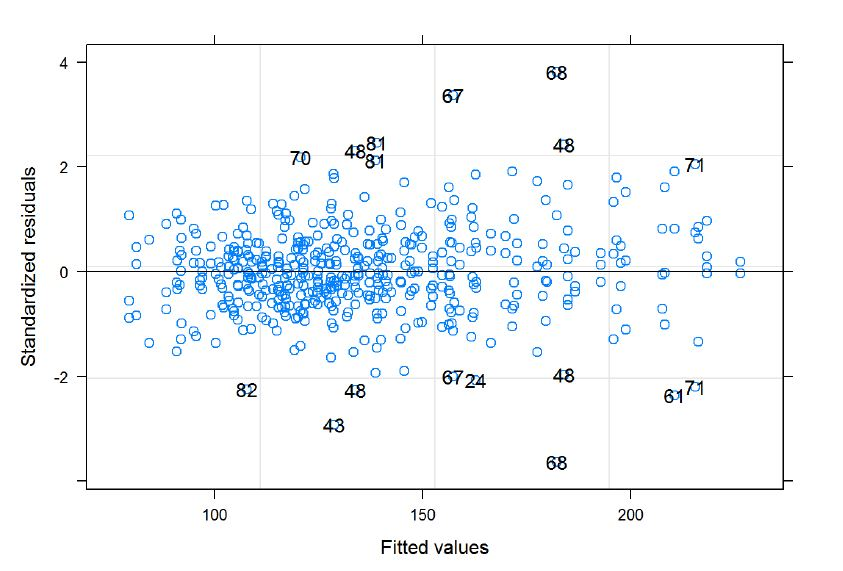
\includegraphics[width=0.9\linewidth]{images/Residuals-JS-Roy}
		\caption{}
		\label{fig:Residuals-JS-Roy}
	\end{figure}
	\subsection{Residual Plots}
	A residual plot is a graph that shows the residuals on the vertical axis and the independent variable on the horizontal axis. If the points in a residual plot are randomly dispersed around the horizontal axis, a linear regression model is appropriate for the data; otherwise, a non-linear model is more appropriate.
	
	\begin{framed}
		\begin{verbatim}
		par(mfrow=c(1,2))
		qqnorm((resid(JS.roy1)[1:255]),
		pch="*",col="red",
		ylim=c(-40,40),
		main="Method J")
		qqline(resid(JS.roy1)[1:255],col="blue")
		qqnorm((resid(JS.roy1)[256:510]),
		pch="*",col="red",
		ylim=c(-40,40),
		main="Method S")
		qqline(resid(JS.roy1)[256:510],col="blue")
		par(mfrow=c(1,1))
		\end{verbatim}	
	\end{framed}
	
	
	\begin{figure}[h!]
		\centering
		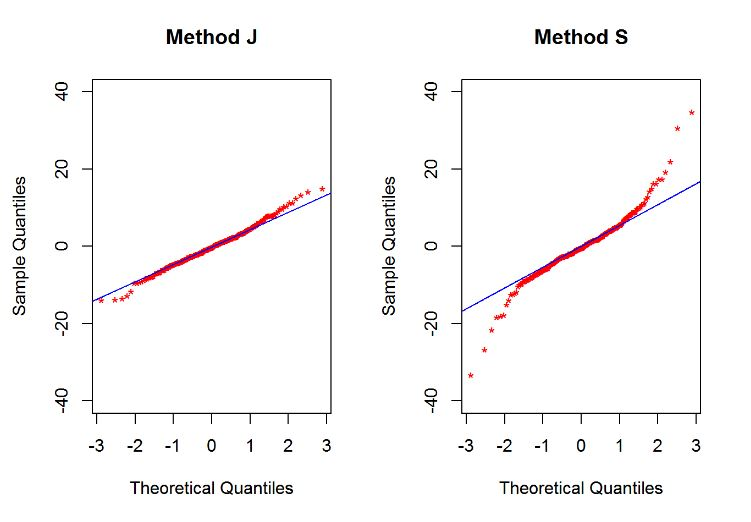
\includegraphics[width=1.1\linewidth]{images/Resid-newplot2}
		\caption{}
		\label{fig:Resid-newplot2}
	\end{figure}
	
	
	\begin{figure}[h!]
		\centering
		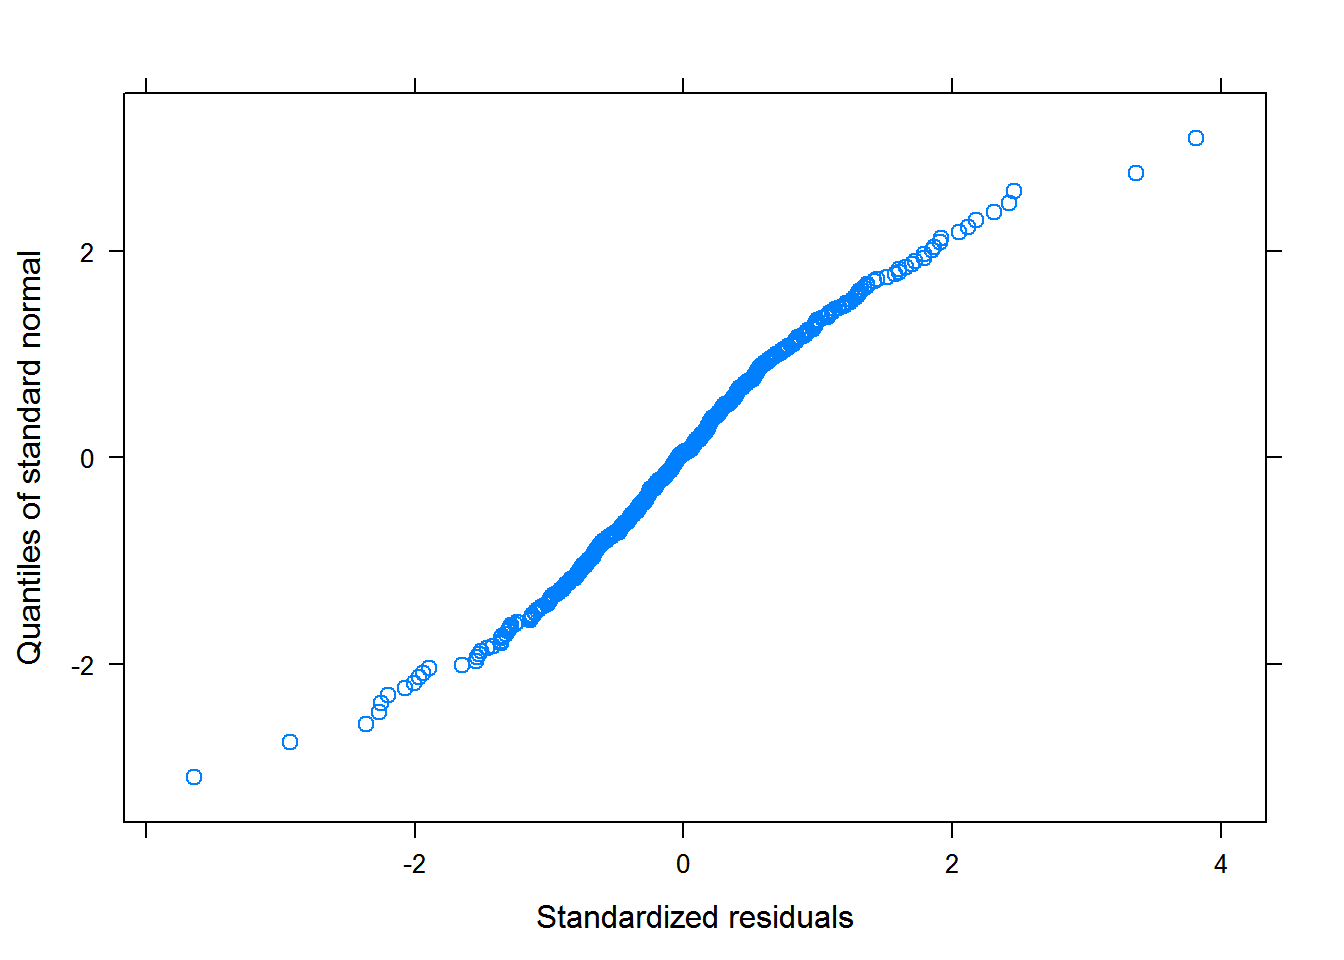
\includegraphics[width=0.9\linewidth]{images/ResidPlot3}
		\label{fig:ResidPlot3}
	\end{figure}
	
	This code will allow you to make QQ plots for each level of the random effects.  LME models assume that not only the within-cluster residuals are normally distributed, but that each level of the random effects are as well. Depending on the model, you can vary the level from 0, 1, 2 and so on
	\begin{framed}
		\begin{verbatim}
		qqnorm(JS.roy1, ~ranef(.))
		
		# 	qqnorm(JS.roy1, ~ranef(.,levels=1)
		\end{verbatim}
	\end{framed}
	\begin{figure}[h!]
		\centering
		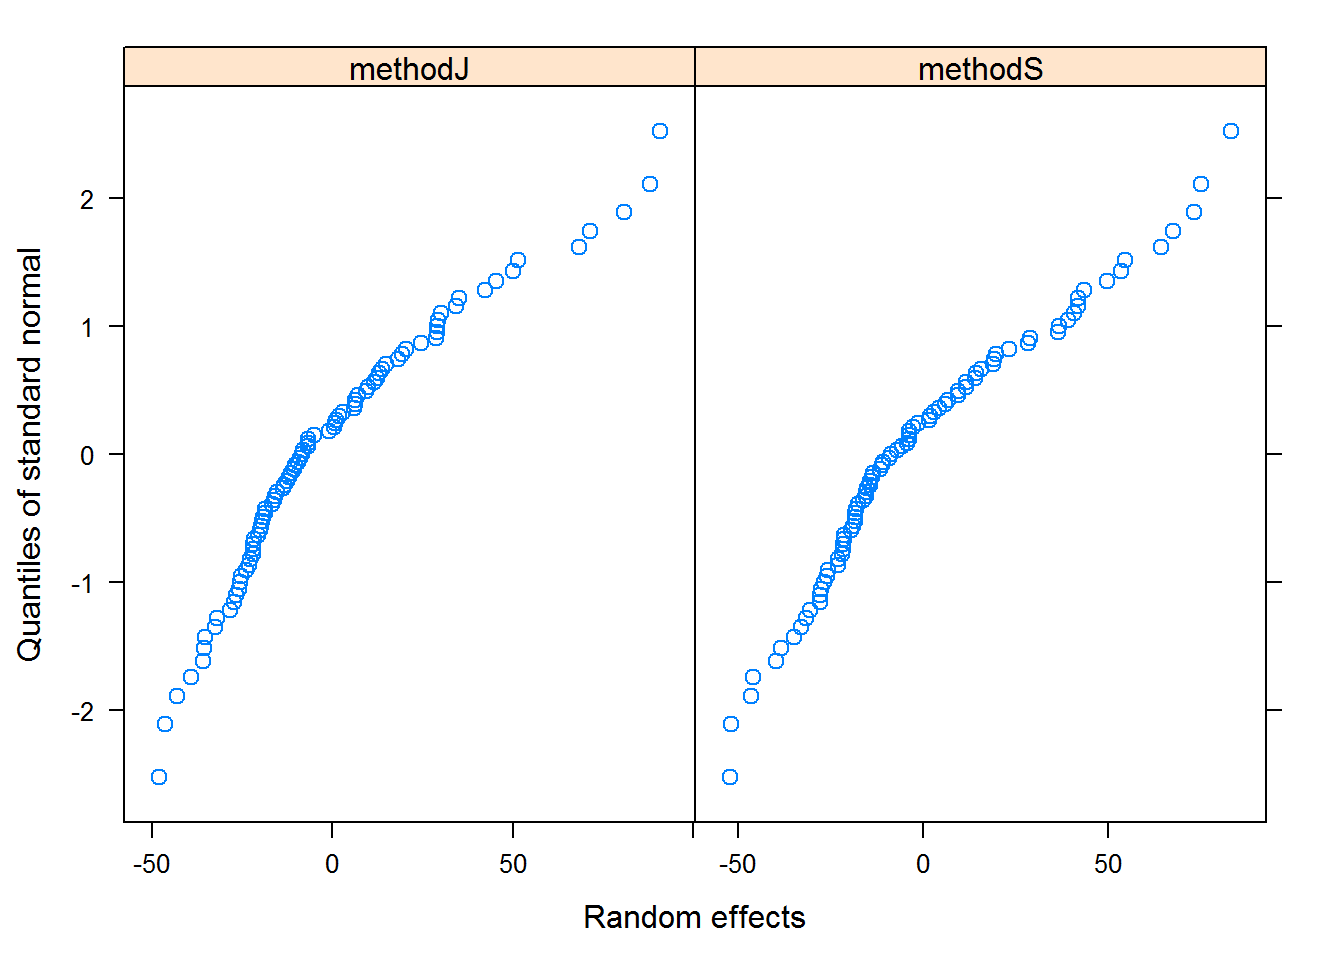
\includegraphics[width=0.9\linewidth]{images/ResidPlot2}
		\caption{}
		\label{fig:ResidPlot2}
	\end{figure}	
\section{Residual Diagnostics}

Consider a residual vector of the form $\hat{e} = \boldsymbol{PY} $, where $\boldsymbol{P}$ is a projection matrix, possibly an oblique projector.
External studentization uses an estimate of $Var$ that does not involve the $i$th observation.
Externally studentized residuals are often preferred over studentized residuals because they have well known distributional
properties in the standard linear models for independent data.
Residuals that are scaled by the estimated variances of the responses are referred to as Pearson-type residuals.
Standardization: \[ \frac{\hat{e}_i}{\sqrt{v_i}}\]
Studentization \[ \frac{\hat{e}_i}{\sqrt{\hat{v}_i}}\]
	\section{Confounded Residuals}
	Hilden-Minton (1995, PhD thesis, UCLA): residual is pure for a specific type of error if it depends only on the fixed components and
	on the error that it is supposed to predict	Residuals that depend on other types of errors are called \textit{\textbf{confounded
			residuals}}
	
	\chapter{Appendices}


	\section{Haslett Hayes}                %-Case Deletion section 3
	
	For fixed effect linear models with correlated error structure
	Haslett (1999) showed that the effects on the fixed effects
	estimate of deleting each observation in turn could be cheaply
	computed from the fixed effects model predicted residuals.
	
	
	A general theory is presented for residuals from the general
	linear model with correlated errors. It is demonstrated that there
	are two fundamental types of residual associated with this model,
	referred to here as the marginal and the conditional residual.
	These measure respectively the distance to the global aspects of
	the model as represented by the expected value and the local
	aspects as represented by the conditional expected value. These
	residuals may be multivariate.
	
	In contrast to classical linear models, diagnostics for LME are
	difficult to perform and interpret, because of the increased
	complexity of the model
	
	%---------------------------------------------------------------------%
\section{RSquared for LME models}
	
	As a complement to this, one can also consider how to properly employ the $R^2$ measure, in the context of Methoc Comparison Studies, further to the work by Edwards et al, namely ``An $R^2$ statistic for fixed effects in the linear mixed model".

	\begin{framed}
		
		\begin{quote}
			\textbf{Abstract for ``An $R^2$ statistic for fixed effects in the linear mixed model"}
			Statisticians most often use the linear mixed model to analyze Gaussian longitudinal data. 
			
			The value and familiarity of the R2 statistic in the linear univariate model naturally creates great interest in extending it to the linear mixed model. We define and describe how to compute a model R2 statistic for the linear mixed model by using only a single model. 
			
			The proposed R2 statistic measures multivariate association between the repeated outcomes and the fixed effects in the linear mixed model. The R2 statistic arises as a 1–1 function of an appropriate F statistic for testing all fixed effects (except typically the intercept) in a full model. 
			
			The statistic compares the full model with a null model with all fixed effects deleted (except typically the intercept) while retaining exactly the same covariance structure. 
			
			Furthermore, the R2 statistic leads immediately to a natural definition of a partial R2 statistic. A mixed model in which ethnicity gives a very small p-value as a longitudinal predictor of blood pressure (BP) compellingly illustrates the value of the statistic. 
			
			In sharp contrast to the extreme p-value, a very small $R^2$ , a measure of statistical and scientific importance, indicates that ethnicity has an almost negligible association with the repeated BP outcomes for the study.
		\end{quote}
	\end{framed}
		
\section{Remarks on the Multivariate Normal Distribution}

Diligence is required when considering the models. Carstensen specifies his models in terms of the univariate normal distribution. Roy's model is specified using the bivariate normal distribution.
This gives rises to a key difference between the two model, in that a bivariate model accounts for covariance between the variables of interest.
The multivariate normal distribution of a $k$-dimensional random vector $X = [X_1, X_2, \ldots, X_k]$
can be written in the following notation:
\[
X\ \sim\ \mathcal{N}(\mu,\, \Sigma),
\]
or to make it explicitly known that $X$ is $k$-dimensional,
\[
X\ \sim\ \mathcal{N}_k(\mu,\, \Sigma).
\]
with $k$-dimensional mean vector
\[ \mu = [ \operatorname{E}[X_1], \operatorname{E}[X_2], \ldots, \operatorname{E}[X_k]] \]
and $k \times k$ covariance matrix
\[ \Sigma = [\operatorname{Cov}[X_i, X_j]], \; i=1,2,\ldots,k; \; j=1,2,\ldots,k \]

\bigskip

\begin{enumerate}
	\item Univariate Normal Distribution
	
	\[
	X\ \sim\ \mathcal{N}(\mu,\, \sigma^2),
	\]
	
	\item Bivariate Normal Distribution
	
	\begin{itemize}
		\item[(a)] \[  X\ \sim\ \mathcal{N}_2(\mu,\, \Sigma), \vspace{1cm}\]
		\item[(b)] \[    \mu = \begin{pmatrix} \mu_x \\ \mu_y \end{pmatrix}, \quad
		\Sigma = \begin{pmatrix} \sigma_x^2 & \rho \sigma_x \sigma_y \\
		\rho \sigma_x \sigma_y  & \sigma_y^2 \end{pmatrix}.\]
	\end{itemize}
\end{enumerate}





\section{Alternative agreement indices}
As an alternative to limits of agreement, \citet{lin2002} proposes the use of
the mean square deviation is assessing agreement. The mean square
deviation is defined as the expectation of the squared differences
of two readings . The MSD is usually used for the case of two
measurement methods $X$ and $Y$ , each making one measurement for
the same subject, and is given by
\[
MSDxy = E[(x - y)^2]  = (\mu_{x} - \mu_{y})^2 + (\sigma_{x} -
\sigma_{y})^2 + 2\sigma_{x}\sigma_{y}(1-\rho_{xy}).
\]


	\citet{Barnhart} advises the use of a predetermined upper limit
	for the MSD value, $MSD_{ul}$, to define satisfactory agreement.
	However, a satisfactory upper limit may not be properly
	determinable, thus creating a drawback to this methodology.
	
	\citet{Barnhart} proposes both the use of the square root of the
	MSD or the expected absolute difference (EAD) as an alternative agreement indices. Both of these indices can be interpreted intuitively, being denominated in the same units of measurements as the original
	measurements. Also they can be compare to the maximum acceptable
	absolute difference between two methods of measurement $d_{0}$.
	\[
	EAD = E(|x - y|) = \frac{\sum |x_{i}- y_{i}|}{n}
	\]
	
	The EAD can be used to supplement the inter-method bias in an
	initial comparison study, as the EAD is informative as a measure
	of dispersion, is easy to calculate and requires no distributional
	assumptions.
	

\citet{Barnhart} remarks that a comparison of EAD and MSD , using
simulation studies, would be interesting, while further adding
that `It will be of interest to investigate the benefits of these
possible new unscaled agreement indices'. For the Grubbs' `F vs C' and `F vs T' comparisons, the inter-method bias, difference variances, limits of agreement and EADs are shown
in Table 1.5. The corresponding Bland-Altman plots for `F vs C' and `F vs T' comparisons were depicted previously on Figure 1.3. While the inter-method bias for the `F vs T' comparison is smaller, the EAD penalizes the comparison for having a greater variance of differences. Hence the EAD values for both comparisons are much closer.

\begin{table}[ht]
		\begin{center}
			\begin{tabular}{|c|c|c|}
				\hline
				& F vs C & F vs T  \\
				\hline
				Inter-method bias & -0.61 & 0.12 3 \\
				Difference variances & 0.06 & 0.22  \\
				Limits of agreement & (-1.08,	-0.13) & (-0.81,1.04) \\
				EAD & 0.61 & 0.35  \\
				\hline
			\end{tabular}
			\caption{Agreement indices for Grubbs' data comparisons.}
		\end{center}
	\end{table}



\section{Coverage Probability}
Further to  \citet{lin2000} and \citet{lin2002}, individual agreement between two measurement methods may be
assessed using the the coverage probability (CP) criteria or the total deviation index (TDI). If $d_{0}$ is predetermined as the maximum acceptable absolute difference between two methods of measurement, the probability that the absolute difference of two measures being less than $d_{0}$ can be computed. This is known as the coverage probability (CP).

\begin{equation}
CP = P(|x_{i} - y_{i}| \leq d_{0})
\end{equation}

If $\pi_{0}$ is set as the predetermined coverage probability, the
boundary under which the proportion of absolute differences is
$\pi_{0}$ may be determined. This boundary is known as the `total
deviation index' (TDI). Hence the TDI is the $100\pi_{0}$
percentile of the absolute difference of paired observations.






	


\section{Basic Models Fits}
Further to \citet{PB}, several simple LME models are constructed
for the blood pressure data. This data set is the subject of a
method comparison study in \citet{BA99}.

\subsection{Implementing the Mixed Models Fits}
They are implemented using the following {\tt{R}} code, utilising the
`nlme' package. An analysis of variance is used to compare the model fits.

The {\tt{R}} script:
\begin{verbatim}
fit1 = lme( BP ~ method, data = dat, random = ~1 | subject )
fit2 = update(fit1, random = ~1 | subject/method )
fit3 = update(fit1, random = ~method - 1 | subject )
#analysis of variance
anova(fit1,fit2,fit3)
\end{verbatim}


\begin{enumerate}
	
	
	\item Simplest workable model, allows differences between methods
	and incorporates a random intercept for each subject. For subject
	1 we have
	\[
	\boldsymbol{X}_i =
	\left(%
	\begin{array}{cc}
	1 & 0 \\
	1 & 0 \\
	1 & 0 \\
	1 & 1 \\
	1 & 1 \\
	1 & 1 \\
	\end{array}%
	\right),\quad
	\boldsymbol{\beta} =
	\left(%
	\begin{array}{c}
	\beta_0 \\
	\beta_1 \\
	\end{array}%
	\right), \quad
	\boldsymbol{Z}_i =
	\left(%
	\begin{array}{c}
	1 \\
	1 \\
	1 \\
	1 \\
	1 \\
	1 \\
	\end{array}%
	\right), \quad \boldsymbol{b}_i = b
	\]
	where $\mathrm{E}(b)=0$ and $\mathrm{var}(b)=\psi.$
	
	\item
	\[
	\boldsymbol{Z}_i =
	\left(%
	\begin{array}{c c}
	1 & 0 \\
	1 & 0 \\
	1 & 0 \\
	0 & 1 \\
	0 & 1 \\
	0 & 1 \\
	\end{array}%
	\right)
	\quad \boldsymbol{b}_i =
	\left(%
	\begin{array}{c c}
	b_1 & 0  \\
	0 & b_2  \\
	\end{array}%
	\right)
	\]
	
	where $\mathrm{E}(b_i)=0$ and $\mathrm{var}(\boldsymbol{b})=
	\boldsymbol{\Psi}$.
	
	The variance of error terms is a $6 \times 6$ matrix.
	
\end{enumerate}




\subsection{Model Fit 1}

This is a simple model with no interactions. There is a fixed effect for each method and a random effect for each subject.
\begin{equation*}
	y_{ijk} = \beta_{j}  + b_{i} + \epsilon_{ijk}, \qquad i=1,\dots,2, j=1,\dots,85, k=1,\dots,3
\end{equation*}

\begin{eqnarray*}
	b_{i} \sim \mathcal{N}(0,\sigma^2_{b}), \qquad \epsilon_{i} \sim \mathcal{N}(0,\sigma^2)
\end{eqnarray*}

\begin{verbatim}
Linear mixed-effects model fit by REML
Data: dat
Log-restricted-likelihood: -2155.853
Fixed: BP ~ method
(Intercept)     methodS
127.40784    15.61961

Random effects:
Formula: ~1 | subject
(Intercept) Residual
StdDev:    29.39085 12.44454

Number of Observations: 510
Number of Groups: 85
\end{verbatim}

The following output was obtained.
\begin{verbatim}
Linear mixed-effects model fit by REML
Data: dat
Log-restricted-likelihood: -2047.582
Fixed: BP ~ method
(Intercept)     methodS
127.40784    15.61961

Random effects:
Formula: ~method - 1 | subject
Structure: General positive-definite, Log-Cholesky parametrization
StdDev    Corr
methodJ  30.455093 methdJ
methodS  31.477237 0.835
Residual  7.763666

Number of Observations: 510
Number of Groups: 85

\end{verbatim}
\newpage
\subsection{Model Fit 1}

This is a simple model with no interactions. There is a fixed effect for each method and a random effect for each subject.
\begin{equation*}
	y_{ijk} = \beta_{j}  + b_{i} + \epsilon_{ijk}, \qquad i=1,\dots,2, j=1,\dots,85, k=1,\dots,3
\end{equation*}

\begin{eqnarray*}
	b_{i} \sim \mathcal{N}(0,\sigma^2_{b}), \qquad \epsilon_{i} \sim \mathcal{N}(0,\sigma^2)
\end{eqnarray*}

\begin{verbatim}
Linear mixed-effects model fit by REML
Data: dat
Log-restricted-likelihood: -2155.853
Fixed: BP ~ method
(Intercept)     methodS
127.40784    15.61961

Random effects:
Formula: ~1 | subject
(Intercept) Residual
StdDev:    29.39085 12.44454

Number of Observations: 510
Number of Groups: 85
\end{verbatim}

The following output was obtained.
\begin{verbatim}
Linear mixed-effects model fit by REML
Data: dat
Log-restricted-likelihood: -2047.582
Fixed: BP ~ method
(Intercept)     methodS
127.40784    15.61961

Random effects:
Formula: ~method - 1 | subject
Structure: General positive-definite, Log-Cholesky parametrization
StdDev    Corr
methodJ  30.455093 methdJ
methodS  31.477237 0.835
Residual  7.763666

Number of Observations: 510
Number of Groups: 85

\end{verbatim}

\newpage
\subsection{Model Fit 2}

This is a simple model, this time with an interaction effect.
There is a fixed effect for each method. This model has random effects at two levels $b_{i}$ for the subject, and
another, $b_{ij}$, for the respective method within each subject.
\begin{equation*}
	y_{ijk} = \beta_{j}  + b_{i} + b_{ij} + \epsilon_{ijk}, \qquad i=1,\dots,2, j=1,\dots,85, k=1,\dots,3
\end{equation*}
\begin{eqnarray*}
	b_{i} \sim \mathcal{N}(0,\sigma^2_{1}), \qquad b_{ij} \sim \mathcal{N}(0,\sigma^2_{2}), \qquad \epsilon_{i} \sim \mathcal{N}(0,\sigma^2)
\end{eqnarray*}

In this model, the random interaction terms all have the same variance $\sigma^2_{2}$. These terms are assumed to be independent of each other, even
within the same subject.

\begin{verbatim}
Linear mixed-effects model fit by REML
Data: dat
Log-restricted-likelihood: -2047.714
Fixed: BP ~ method
(Intercept)     methodS
127.40784    15.61961

Random effects:
Formula: ~1 | subject
(Intercept)
StdDev:    28.28452

Formula: ~1 | method %in% subject
(Intercept) Residual
StdDev:    12.61562 7.763666

Number of Observations: 510
Number of Groups:
subject method %in% subject
85                 170
\end{verbatim}
\newpage
\subsection{Model Fit 3}

This model is a more general model, compared to 'model fit 2'. This model treats the random interactions for each subject as a vector and
allows the variance-covariance matrix for that vector to be estimated from the set of all positive-definite matrices.
$\boldsymbol{y_{i}}$ is the entire response vector for the $i$th subject.
$\boldsymbol{X_{i}}$ and $\boldsymbol{Z_{i}}$  are the fixed- and random-effects design matrices respectively.
\begin{equation*}
	\boldsymbol{y_{i}} = \boldsymbol{X_{i}\beta}  + \boldsymbol{Z_{i}b_{i}} + \boldsymbol{\epsilon_{i}}, \qquad i=1,\dots,85
\end{equation*}
\begin{eqnarray*}
	\boldsymbol{Z_{i}} \sim \mathcal{N}(\boldsymbol{0,\Psi}),\qquad
	\boldsymbol{\epsilon_{i}} \sim \mathcal{N}(\boldsymbol{0,\sigma^2\Lambda})
\end{eqnarray*}

For the first subject the response vector, $\boldsymbol{y_{1}}$, is:
\begin{table}[ht]
	\begin{center}
		\begin{tabular}{rrllr}
			\hline
			observation & BP & subject & method & replicate \\
			\hline
			1 & 100.00 & 1 & J &   1 \\
			86 & 106.00 & 1 & J &   2 \\
			171 & 107.00 & 1 & J &   3 \\
			511 & 122.00 & 1 & S &   1 \\
			596 & 128.00 & 1 & S &   2 \\
			681 & 124.00 & 1 & S &   3 \\
			\hline
		\end{tabular}
	\end{center}
\end{table}
\newpage
The fixed effects design matrix $\boldsymbol{X_{i}}$ is given by:
\begin{table}[ht]
	\begin{center}
		\begin{tabular}{r|r}
			\hline
			(Intercept) & method S \\
			\hline
			1 & 0 \\
			1 & 0 \\
			1 & 0 \\
			1 & 1 \\
			1 & 1 \\
			1 & 1 \\
			\hline
		\end{tabular}
	\end{center}
\end{table}

\newpage




The random effects design matrix $\boldsymbol{Z_{i}}$ is given by:
\begin{table}[ht]
	\begin{center}
		\begin{tabular}{r|r}
			\hline
			method J & method S \\
			\hline
			1 & 0 \\
			1 & 0 \\
			1 & 0 \\
			0 & 1 \\
			0 & 1 \\
			0 & 1 \\
			\hline
		\end{tabular}
	\end{center}
\end{table}
\newpage

\subsection{Using LME models to create Prediction Intervals}
\citet{BXC2004} also advocates the use of linear mixed models in
the study of method comparisons. The model is constructed to
describe the relationship between a value of measurement and its
real value. The non-replicate case is considered first, as it is
the context of the Bland Altman plots. This model assumes that
inter-method bias is the only difference between the two methods.
A measurement $y_{mi}$ by method $m$ on individual $i$ is
formulated as follows;
\begin{equation}
	y_{mi}  = \alpha_{m} + \mu_{i} + e_{mi} \qquad ( e_{mi} \sim
	N(0,\sigma^{2}_{m}))
\end{equation}
The differences are expressed as $d_{i} = y_{1i} - y_{2i}$ For the
replicate case, an interaction term $c$ is added to the model,
with an associated variance component. All the random effects are
assumed independent, and that all replicate measurements are
assumed to be exchangeable within each method.

\begin{equation}
	y_{mir}  = \alpha_{m} + \mu_{i} + c_{mi} + e_{mir} \qquad ( e_{mi}
	\sim N(0,\sigma^{2}_{m}), c_{mi} \sim N(0,\tau^{2}_{m}))
\end{equation}

\citet{BXC2008} proposes a methodology to calculate prediction
intervals in the presence of replicate measurements, overcoming
problems associated with Bland-Altman methodology in this regard.
It is not possible to estimate the interaction variance components
$\tau^{2}_{1}$ and $\tau^{2}_{2}$ separately. Therefore it must be
assumed that they are equal. The variance of the difference can be
estimated as follows:
\begin{equation}
	var(y_{1j}-y_{2j})
\end{equation}

\subsection{Computation} Modern software
packages can be used to fit models accordingly. The best linear
unbiased predictor (BLUP) for a specific subject $i$ measured with
method $m$ has the form $BLUP_{mir} = \hat{\alpha_{m}} +
\hat{\beta_{m}}\mu_{i} + c_{mi}$, under the assumption that the
$\mu$s are the true item values.





\section{Demonstration of Roy's testing}
Roy provides three case studies, using data sets well known in method comparison studies, to demonstrate how the methodology should be used. The first two examples used are from the `blood pressure' data set introduced by \citet{BA99}. The data set is a tabulation of simultaneous measurements of systolic blood pressure were made by each of two experienced observers (denoted `J' and `R') using a sphygmomanometer and by a semi-automatic blood pressure monitor (denoted `S'). Three sets of readings were made in quick succession. Roy compares the `J' and `S' methods in the first of her examples.

The inter-method bias between the two method is found to be $15.62$ , with a $t-$value of $-7.64$, with a $p-$value of less than $0.0001$. Consequently there is a significant inter-method bias present between methods $J$ and $S$, and the first of the Roy's three agreement criteria is unfulfilled.

Next, the first variability test is carried out, yielding maximum likelihood estimates of the between-subject variance covariance matrix, for both the null model, in compound symmetry (CS) form, and the alternative model in symmetric (symm) form. These matrices are determined to be as follows;
\[
\boldsymbol{\hat{D}}_{CS} = \left( \begin{array}{cc}
946.50 & 784.32  \\
784.32 & 946.50  \\
\end{array}\right),
\hspace{1.5cm}
\boldsymbol{\hat{D}}_{Symm} = \left( \begin{array}{cc}
923.98 & 785.24  \\
785.24 & 971.30  \\
\end{array}\right).
\]

A likelihood ratio test is perform to compare both candidate models. The log-likelihood of the null model is $-2030.7$, and for the alternative model $-2030.8$. The test statistic, presented with greater precision than the log-likelihoods, is $0.1592$. The $p-$value is $0.6958$. Consequently we fail to reject the null model, and by extension, conclude that the hypothesis that methods $J$ and $S$ have the same between-subject variability. Thus the second of the criteria is fulfilled.

The second variability test determines maximum likelihood estimates of the within-subject variance covariance matrix, for both the null model, in CS form, and the alternative model in symmetric form.

\[
\boldsymbol{\hat{\Lambda}_{CS}} = \left( \begin{array}{cc}
60.27  & 16.06  \\
16.06  & 60.27  \\
\end{array}\right),
\hspace{1.5cm}
\boldsymbol{\hat{\Lambda}}_{Symm} = \left( \begin{array}{cc}
37.40 & 16.06  \\
16.06 & 83.14  \\
\end{array}\right).
\]

Again, A likelihood ratio test is perform to compare both candidate models. The log-likelihood of the alternative model model is $-2045.0$. As before, the null model has a log-likelihood of $-2030.7$. The test statistic is computed as $28.617$, again presented with greater precision. The $p-$value is less than $0.0001$. In this case we reject the null hypothesis of equal within-subject variability. Consequently the third of Roy's criteria is unfulfilled.
The coefficient of repeatability for methods $J$ and $S$ are found to be 16.95 mmHg and 25.28 mmHg respectively.

The last of the three variability tests is carried out to compare the overall variabilities of both methods.
With the null model the MLE of the within-subject variance covariance matrix is given below. The overall variabilities for the null and alternative models, respectively, are determined to be as follows;
\[
\boldsymbol{\hat{\Sigma}}_{CS} = \left( \begin{array}{cc}
1007.92  & 801.65  \\
801.65  & 1007.92  \\
\end{array}\right),
\hspace{1.5cm}
\boldsymbol{\hat{\Sigma}}_{Symm} = \left( \begin{array}{cc}
961.38 & 801.40  \\
801.40 & 1054.43  \\
\end{array}\right),
\]

The log-likelihood of the alternative model model is $-2045.2$, and again, the null model has a log-likelihood of $-2030.7$. The test statistic is $28.884$, and the $p-$value is less than $0.0001$. The null hypothesis, that both methods have equal overall variability, is rejected. Further to the second variability test, it is known that this difference is specifically due to the difference of within-subject variabilities.

Lastly, Roy considers the overall correlation coefficient. The diagonal blocks $\boldsymbol{\hat{r}_{\Omega}}_{ii}$ of the correlation matrix indicate an overall coefficient of $0.7959$. This is less than the threshold of 0.82 that Roy recommends.

\[
\boldsymbol{\hat{r}_{\Omega}}_{ii} = \left( \begin{array}{cc}
1  & 0.7959  \\
0.7959  & 1  \\
\end{array}\right)
\]

The off-diagonal blocks of the overall correlation matrix $\boldsymbol{\hat{r}_{\Omega}}_{ii'}$ present the correlation coefficients further to \citet{hamlett}.
\[
\boldsymbol{\hat{r}_{\Omega}}_{ii'} = \left( \begin{array}{cc}
0.9611  & 0.7799  \\
0.7799  & 0.9212  \\
\end{array}\right).
\]

The overall conclusion of the procedure is that method $J$ and $S$ are not in agreement, specifically due to the within-subject variability, and the inter-method bias. The repeatability coefficients are substantially different, with the coefficient for method $S$ being 49\% larger than for method $J$. Additionally the overall correlation coefficient did not exceed the recommended threshold of $0.82$.


%========================================================= %
%% %% - Part E- Part E

\section{Demonstration of Roy's testing}
Roy provides three case studies, using data sets well known in method comparison studies, to demonstrate how the methodology should be used. The first two examples used are from the `blood pressure' data set introduced by \citet{BA99}. The data set is a tabulation of simultaneous measurements of systolic blood pressure were made by each of two experienced observers (denoted `J' and `R') using a sphygmomanometer and by a semi-automatic blood pressure monitor (denoted `S'). Three sets of readings were made in quick succession. Roy compares the `J' and `S' methods in his first example, and the `R' and `S' methods in his second.



%--------------------------------------------------%
\subsection{Matrix structures}
Before discussing the tests, it is useful to point out the difference between symmetric form and compound symmetry form. Consider a generic matrix $A$,

\begin{equation}
\boldsymbol{A} = \left( \begin{array}{cc}
a_{11} & a_{12}  \\
a_{21} & a_{22}  \\
\end{array}\right).
\end{equation}

A symmetric matrix allows the diagonal terms $a_{11}$ and $a_{22}$ to differ.
The compound symmetry structure requires that both of these terms be equal, i.e $a_{11} = a_{22}$.

%--------------------------------------------------%
\subsection{Variability test 1}
This is a test on whether both methods $A$ and $B$ have the same between-subject variability or not.
\begin{eqnarray}
H_{0}: \mbox{ }d_{A}  = d_{B} \\
H_{A}: \mbox{ }d_{A}  \neq d_{B}
\end{eqnarray}
When implemented using \texttt{R}, this test is facilitated by constructing a model specifying a symmetric form for $D$ (i.e. the alternative model) and comparing it with a model that has compound symmetric form for $D$ (i.e. the null model). For this test $\boldsymbol{\hat{\Lambda}}$ has a symmetric form for both models, and will be the same for both.

%--------------------------------------------------%
\subsubsection{Bland-Altman's blood data}
With the alternative model, the MLE of the between-subject variance covariance matrix is given by
\begin{equation}
\boldsymbol{\hat{D}_{Symm}} = \left( \begin{array}{cc}
923.98 & 785.24  \\
785.24 & 971.30  \\
\end{array}\right)
\end{equation}

With the null model the MLE is as follows:

\begin{equation}
\boldsymbol{\hat{D}_{CS}} = \left( \begin{array}{cc}
946.50 & 784.32  \\
784.32 & 946.50  \\
\end{array}\right)
\end{equation}
A likelihood ratio test is perform to determine which model is more suitable. The outcome of this test is presented in the following \texttt{R} code.
\begin{verbatim}
> anova(MCS1,MCS2)
>
>
Model df    AIC    BIC  logLik   Test L.Ratio p-value
MCS1     1  8 4077.5 4111.3 -2030.7
MCS2     2  7 4075.6 4105.3 -2030.8 1 vs 2 0.15291  0.6958
\end{verbatim}

The test statistic is the difference of the $-2$ log likelihoods; $0.15291$. The $p-$value is $0.6958$. Therefore we fail to reject the hypothesis that both have the same between-subject variabilities.

%---------------------------------------------%
\subsection{Variability test 2}

This is a test on whether both methods $A$ and $B$ have the same within-subject variability or not.

\begin{eqnarray}
H_{0}: \mbox{ }\lambda_{A}  = \lambda_{B} \\
H_{A}: \mbox{ }\lambda_{A}  = \lambda_{B}
\end{eqnarray}

This model is performed in the same manner as the first test, only reversing the roles of $\boldsymbol{\hat{D}}$ and $\boldsymbol{\hat{\Lambda}}$. The null model is constructed  a symmetric form for $\boldsymbol{\hat{\Lambda}}$ while the alternative model uses a compound symmetry form. This time $\boldsymbol{\hat{D}}$ has a symmetric form for both models, and will be the same for both.


\subsubsection{Bland-Altman's blood data}
For the null model the MLE of the within-subject variance covariance matrix is given below.

\begin{equation}
\boldsymbol{\hat{\Lambda}_{Symm}} = \left( \begin{array}{cc}
37.40 & 16.06  \\
16.06 & 83.14  \\
\end{array}\right)
\end{equation}
With the alternative model the MLE is as follows:

\begin{equation}
\boldsymbol{\hat{\Lambda}_{CS}} = \left( \begin{array}{cc}
60.27  & 16.06  \\
16.06  & 60.27  \\
\end{array}\right)
\end{equation}

A likelihood ratio test is perform to determine which model is more suitable.
The outcome of this test is that it can be assumed that they have equal
The test statistic is the difference of the $-2$ log likelihoods; $28.617$. The $p-$value is less than $0.0001$. In this case we reject the null hypothesis that both models have the same within-subject variabilities.

%-----------------------------------------------%
\subsection{Variability test 3}
This is a test on whether both methods $A$ and $B$ have the same overall variability or not.
\begin{eqnarray}
H_{0}: \mbox{ }\sigma_{A}  = \sigma_{B} \\
H_{A}: \mbox{ }\sigma_{A}  = \sigma_{B}
\end{eqnarray}

The null model is constructed a symmetric form for both $\boldsymbol{\hat{D}}$ and $\boldsymbol{\hat{\Lambda}}$ while the alternative model uses a compound symmetry form for both.

\subsubsection{Bland-Altman's blood data}
With the null model the MLE of the within-subject variance covariance matrix is given below.

\begin{equation}
\boldsymbol{\hat{\Sigma}_{Symm}} = \left( \begin{array}{cc}
961.38 & 801.40  \\
801.40 & 1054.43  \\
\end{array}\right)
\end{equation}

With the alternative model the MLE is as follows:
\begin{equation}
\boldsymbol{\hat{\Sigma}_{CS}} = \left( \begin{array}{cc}
1007.92  & 801.65  \\
801.65  & 1007.92  \\
\end{array}\right)
\end{equation}

Again a likelihood ratio test is used to determine the most suitable of the two candidate models.
The test statistic is the difference of the $-2$ log likelihoods; $28.884$. The $p-$value is less than $0.0001$. We again reject the null hypothesis. Each model has a different overall variability, a foregone conclusion from the second variability test.



\subsection{Test for inter-method bias}
The inter-method bias between the two method is found to be $15.62$ , with a $p-$value of

\subsection{Correlation Test}
\begin{equation}
\boldsymbol{\hat{r}_{\Omega}}_{ii} = \left( \begin{array}{cc}
1  & 0.7959  \\
0.7959  & 1  \\
\end{array}\right)
\end{equation}

The  diagonal blocks $\boldsymbol{\hat{r}_{\Omega}}_{ii}$ of the correlation matrix indicate an overall coefficient of $0.7959$.
This is less than the threshold of 0.82 that Roy recommends.

The off diagonal blocks of the overall correlation matrix $\boldsymbol{\hat{r}_{\Omega}}_{ii'}$ are
\begin{equation}
\boldsymbol{\hat{r}_{\Omega}}_{ii'} = \left( \begin{array}{cc}
0.9611  & 0.7799  \\
0.7799  & 0.9212  \\
\end{array}\right).
\end{equation}

\subsection{Conclusion of procedure}
The overall conclusion of the procedure is that the two methods are not in agreement, specifically due to the within-subject variability, and the inter-method bias. The repeatability coefficients are substantially different, one being 49\% larger than the other. Additionally the overall correlation coefficient did not exceed the recommended threshold of $0.82$.

%------------------------------------------------------------------------------------%
\newpage

\section*{Using Roy's Test to Identify cause of Lack of agreement}

Barnhart specifies three conditions for method of measurement that are required for two methods of measurement to be considered in agreement.

\begin{itemize}
	\item[(i)] No Significant Inter-method bias
	\item[(ii)] No significant Difference in Within-Subject Variance
	\item[(iii)] No significant Difference in Within-Subject Variance 
\end{itemize}


Roy(2009) demonstrates a LME model specification, and a series of tests that look at each of these agreement criteria individually. If two methods of measuement lack agreement, the specific reason or reasons for this lack of agreement can be identified.


Roy proposes an LME model with Kronecker product covariance structure in a doubly multivariate setup. Response for $i$th subject can be written as
\[ y_i = \beta_0 + \beta_1x_{i1} + \beta_2x_{i2} + b_{1i}z_{i1}  + b_{2i}z_{i2} + \epsilon_i \]
\begin{itemize}
	\item $\beta_1$ and $\beta_2$ are fixed effects corresponding to both methods. ($\beta_0$ is the intercept.)
	\item $b_{1i}$ and $b_{2i}$ are random effects corresponding to both methods.
\end{itemize}

Overall variability between the two methods ($\Omega$) is sum of between-subject ($D$) and within-subject variability ($\Sigma$),
\[
\mbox{Block } \boldsymbol{\Omega}_i = \left[ \begin{array}{cc} d^2_1 & d_{12}\\ d_{12} & d^2_2\\ \end{array} \right]
+ \left[\begin{array}{cc} \sigma^2_1 & \sigma_{12}\\ \sigma_{12} & \sigma^2_2\\ \end{array}\right].
\]
%============================================== %
%- F:

\section*{Using Roy's Model to Compute LoAs and CR }

In this short section, a demonstration of how Roy's technique can be used to compute two common MCS metrics: Limits of Agreement and the Coefficient of Repeatabilty. While Limits of Agreement are not used in the analysis proposed here, they are ubiquituous in literature, and a demonstration on how to compute them with the Roy Model would assist the adoption of this proposed method.

The coefficient of repeatability is encountered in Gage R \& R analysis. \textit{(A future exploration of how LME models can be used in that field would be of interest. This is something to include in the Conclusions Section).}
%======================
\section{Worked Eamples : LikelihoodRatio Tests}

Conventionally LME models can be tested using Likelihood Ratio Tests, wherein a reference model is compared to a nested model.
\begin{framed}
	\begin{verbatim}
	> Ref.Fit = lme(y ~ meth-1, data = dat,   #Symm , Symm#
	+     random = list(item=pdSymm(~ meth-1)), 
	+     weights=varIdent(form=~1|meth),
	+     correlation = corSymm(form=~1 | item/repl), 
	+     method="ML")
	\end{verbatim}
\end{framed}
Roy(2009) presents two nested models that specify the condition of equality as required, with a third nested model for an additional test. There three formulations share the same structure, and can be specified by making slight alterations of the code for the Reference Model.
Nested Model (Between-Item Variability)
\begin{framed}
	\begin{verbatim}
	> NMB.fit  = lme(y ~ meth-1, data = dat,   #CS , Symm#
	+     random = list(item=pdCompSymm(~ meth-1)),
	+     correlation = corSymm(form=~1 | item/repl), 
	+     method="ML")
	\end{verbatim}
\end{framed}



\begin{framed}
	\begin{verbatim}
	Nested Model (Within ?item Variability)
	> NMW.fit = lme(y ~ meth-1, data = dat,   #Symm , CS# 
	+     random = list(item=pdSymm(~ meth-1)),
	+     weights=varIdent(form=~1|meth), 
	+     correlation = corCompSymm(form=~1 | item/repl), 
	+     method="ML")
	\end{verbatim}
\end{framed}

Nested Model (Overall Variability)
Additionally there is a third nested model, that can be used to test overall variability, substantively a a joint test for between-item and within-item variability. The motivation for including such a test in the suite is not clear, although it does circumvent the need for multiple comparison procedures in certain circumstances, hence providing a simplified procedure for non-statisticians.

\begin{framed}
	\begin{verbatim}
	> NMO.fit = lme(y ~ meth-1, data = dat,   #CS , CS# 
	+     random = list(item=pdCompSymm(~ meth-1)), 
	+     correlation = corCompSymm(form=~1 | item/repl), 
	+     method="ML")
	\end{verbatim}
\end{framed}

ANOVAs  for  Original Fits
The likelihood Ratio test is very simple to implement in R. All that is required it to specify the reference model and the relevant nested mode as arguments to the command anova().
The figure below displays the three tests described by Roy (2009).

\begin{framed}
	\begin{verbatim}
	> testB    = anova(Ref.Fit,NMB.fit)                          # Between-Subject Variabilities
	> testW   = anova(Ref.Fit,NMW.fit)                        # Within-Subject Variabilities
	> testO     = anova(Ref.Fit,NMO.fit)                        # Overall Variabilities
	
	\end{verbatim}
\end{framed}




%-----------------------------------------------------------------------------------------------------%
\newpage



\newpage   
\begin{verbatim}
> anova(MCS1,MCS2)
>
>
Model df    AIC    BIC  logLik   Test L.Ratio p-value
MCS1     1  8 4077.5 4111.3 -2030.7
MCS2     2  7 4075.6 4105.3 -2030.8 1 vs 2 0.15291  0.6958
\end{verbatim}

\subsection{Roy's Reference Model}
Conventionally LME models can be tested using Likelihood Ratio Tests, wherein a reference model is compared to a nested model.
\begin{framed}
	\begin{verbatim}
	> Ref.Fit = lme(y ~ meth-1, data = dat,   #Symm , Symm#
	+     random = list(item=pdSymm(~ meth-1)), 
	+     weights=varIdent(form=~1|meth),
	+     correlation = corSymm(form=~1 | item/repl), 
	+     method="ML")
	\end{verbatim}
\end{framed}


Roy(2009) presents two nested models that specify the condition of equality as required, with a third nested model for an additional test. There three formulations share the same structure, and can be specified by making slight alterations of the code for the Reference Model.

\subsection{Nested Model (Between-Item Variability)}
\begin{framed}
	\begin{verbatim}
	> NMB.fit  = lme(y ~ meth-1, data = dat,   #CS , Symm#
	+     random = list(item=pdCompSymm(~ meth-1)),
	+     correlation = corSymm(form=~1 | item/repl), 
	+     method="ML")
	\end{verbatim}
\end{framed}


\newpage
\section{Fat Data Examples: LoAs for Carstensen's data}




\citet{BXC2008} presents a data set `fat', which is a comparison of measurements of subcutaneous fat
by two observers at the Steno Diabetes Center, Copenhagen. Measurements are in millimeters
(mm). Each person is measured three times by each observer. The observations are considered to be `true' replicates.

A linear mixed effects model is formulated, and implementation through several software packages is demonstrated.
All of the necessary terms are presented in the computer output. The limits of agreement are therefore,
\begin{equation}
0.0449  \pm 1.96 \times  \sqrt{2 \times 0.0596^2 + 0.0772^2 + 0.0724^2} = (-0.220,  0.309).
\end{equation}

\citet{BXC2008} describes the calculation of the limits of agreement (with the inter-method bias implicit) for both data sets, based on his formulation;

\[\hat{\alpha}_1 - \hat{\alpha}_2 \pm 2\sqrt{2\hat{\tau}^2 +\hat{\sigma}_1^2 +\hat{\sigma}_2^2 }.\]

For the `Fat' data set, the inter-method bias is shown to be $0.045$. The limits of agreement are $(-0.23 , 0.32)$



For Carstensen's `fat' data, the limits of agreement computed using Roy's
method are consistent with the estimates given by \citet{BXC2008}; $0.044884  \pm 1.96 \times  0.1373979 = (-0.224,  0.314).$






\section{HBA1C Diabetes Example}
\citet{BXC2008} describes the sampling method when discussing of a motivating example

Diabetes patients attending an outpatient clinic in Denmark have their $HbA_{1c}$ levels routinely measured at every visit. Venous and Capillary blood samples were obtained from all patients appearing at the clinic over two days. Samples were measured on four consecutive days on each machines, hence there are five analysis days.

\citet{BXC2008} notes that every machine was calibrated every day to  the manufacturers guidelines.
Measurements are classified by method, individual and replicate. In this case the replicates are clearly not exchangeable, neither within patients nor simulataneously for all patients.


%	\citet{Roy2006} uses the ``Blood" data set, which featured in \citet{BA99}.

%=========================================================================== %
\section{Oximetry Data}
\citet{BXC2008} introduces a second data set; the oximetry study. This study done at the Royal Children�s Hospital in
Melbourne to assess the agreement between co-oximetry and pulse oximetry in small babies.

In most cases, measurements were taken by both method at three different times. In some cases there are either one or two pairs of measurements, hence the data is unbalanced. \citet{BXC2008} describes many of the children as being very sick, and with very low oxygen saturations levels. Therefore it must be assumed that a biological change can occur in interim periods, and measurements are not true replicates.

\citet{BXC2008} proposes the addition of an random effects term to their model when the replicates are linked. This term is used to describe the `item by replicate' interaction, which is independent of the methods. This interaction is a source of variability independent of the methods. Therefore failure to account for it will result in variability being wrongly attributed to the methods.

%=========================================================================== %

Limits of agreement are determined using Roy's methodology, without adding any additional terms, are found to be consistent with the `interaction' model; $(-9.562, 14.504 )$. Roy's methodology assumes that replicates are linked. However, following Carstensen's example, an addition interaction term is added to the implementation of Roy's model to assess the effect, the limits of agreement estimates do not change. However there is a conspicuous difference in within-subject matrices of Roy's model and the modified model (denoted $1$ and $2$ respectively);

Carstensen demonstrates the use of the interaction term when computing the limits of agreement for the `Oximetry' data set. When the interaction term is omitted, the limits of agreement are $(-9.97, 14.81)$. Carstensen advises the inclusion of the interaction term for linked replicates, and hence the limits of agreement are recomputed as $(-12.18,17.12)$.


Limits of agreement are determined using Roy's methodology, without adding any additional terms, are found to be consistent with the `interaction' model; $(-9.562, 14.504 )$. Roy's methodology assumes that replicates are linked. However, following Carstensen's example, an addition interaction term is added to the implementation of Roy's model to assess the effect, the limits of agreement estimates do not change. However there is a conspicuous difference in within-subject matrices of Roy's model and the modified model (denoted $1$ and $2$ respectively);
%	\begin{equation}
%	\hat{\boldsymbol{\Lambda}}_{1}= \begin{pmatrix}{
%		16.61 &	11.67\cr
%		11.67 & 27.65 }\qquad
%	\boldsymbol{\hat{\Lambda}}_{2}= \begin{pmatrix}{
%		7.55 & 2.60 \cr
%		2.60 & 18.59}.
%	\end{equation}

\noindent (The variance of the additional random effect in model $2$ is $3.01$.)

\citet{akaike} introduces the Akaike information criterion ($AIC$), a model
selection tool based on the likelihood function. Given a data set, candidate models
are ranked according to their AIC values, with the model having the lowest AIC being considered the best fit.Two candidate models can said to be equally good if there is a difference of less than $2$ in their AIC values.

The Akaike information criterion (AIC) for both models are $AIC_{1} = 2304.226$ and $AIC_{2} = 2306.226$ , indicating little difference in models. The AIC values for the Carstensen `unlinked' and `linked' models are $1994.66$ and $1955.48$ respectively, indicating an improvement by adding the interaction term.

The $\boldsymbol{\hat{\Lambda}}$ matrices are informative as to the difference between Carstensen's unlinked and linked models. For the oximetry data, the covariance terms (given above as 11.67 and 2.6 respectively ) are of similar magnitudes to the variance terms. Conversely for the `fat' data the covariance term ($-0.00032$) is negligible. When the interaction term is added to the model, the covariance term remains negligible. (For the `fat' data, the difference in AIC values is also approximately $2$).

To conclude, Carstensen's models provided a rigorous way to determine limits of agreement, but don't provide for the computation of $\boldsymbol{\hat{D}}$ and $\boldsymbol{\hat{\Lambda}}$. Therefore the test's proposed by \citet{ARoy2009} can not be implemented. Conversely, accurate limits of agreement as determined by Carstensen's model may also be found using Roy's method. Addition of the interaction term erodes the capability of Roy's methodology to compare candidate models, and therefore shall not be adopted.

Finally, to complement the blood pressure (i.e.`J vs S') method comparison from the previous section (i.e.`J vs S'), the limits of agreement are $15.62 \pm 1.96 \times 20.33 = (-24.22, 55.46)$.)



\section{Linked replicates}

\citet{BXC2008} proposes the addition of an random effects term to their model when the replicates are linked. This term is used to describe the `item by replicate' interaction, which is independent of the methods. This interaction is a source of variability independent of the methods. Therefore failure to account for it will result in variability being wrongly attributed to the methods.

\citet{BXC2008} introduces a second data set; the oximetry study. This study done at the Royal Children�s Hospital in
Melbourne to assess the agreement between co-oximetry and pulse oximetry in small babies.

In most cases, measurements were taken by both method at three different times. In some cases there are either one or two pairs of measurements, hence the data is unbalanced. \citet{BXC2008} describes many of the children as being very sick, and with very low oxygen saturations levels. Therefore it must be assumed that a biological change can occur in interim periods, and measurements are not true replicates.

Limits of agreement are determined using Roy's methodology, without adding any additional terms, are found to be consistent with the `interaction' model; $(-9.562, 14.504 )$. Roy's methodology assumes that replicates are linked. However, following Carstensen's example, an addition interaction term is added to the implementation of Roy's model to assess the effect, the limits of agreement estimates do not change. However there is a conspicuous difference in within-subject matrices of Roy's model and the modified model (denoted $1$ and $2$ respectively);
\begin{equation}
	\hat{\boldsymbol{\Lambda}}_{1}= \left(\begin{array}{cc}
		16.61 &	11.67\\
		11.67 & 27.65 \end{array}\right) \qquad
	\boldsymbol{\hat{\Lambda}}_{2}= \left( \begin{array}{cc}
		7.55 & 2.60 \\
		2.60 & 18.59 \end{array} \right).
\end{equation}

\noindent (The variance of the additional random effect in model $2$ is $3.01$.)

\citet{akaike} introduces the Akaike information criterion ($AIC$), a model
selection tool based on the likelihood function. Given a data set, candidate models
are ranked according to their AIC values, with the model having the lowest AIC being considered the best fit.Two candidate models can said to be equally good if there is a difference of less than $2$ in their AIC values.

The Akaike information criterion (AIC) for both models are $AIC_{1} = 2304.226$ and $AIC_{2} = 2306.226$ , indicating little difference in models. The AIC values for the Carstensen `unlinked' and `linked' models are $1994.66$ and $1955.48$ respectively, indicating an improvement by adding the interaction term.

The $\boldsymbol{\hat{\Lambda}}$ matrices are informative as to the difference between Carstensen's unlinked and linked models. For the oximetry data, the covariance terms (given above as 11.67 and 2.6 respectively ) are of similar magnitudes to the variance terms. Conversely for the `fat' data the covariance term ($-0.00032$) is negligible. When the interaction term is added to the model, the covariance term remains negligible. (For the `fat' data, the difference in AIC values is also approximately $2$).

To conclude, Carstensen's models provided a rigorous way to determine limits of agreement, but don't provide for the computation of $\boldsymbol{\hat{D}}$ and $\boldsymbol{\hat{\Lambda}}$. Therefore the test's proposed by \citet{roy} can not be implemented. Conversely, accurate limits of agreement as determined by Carstensen's model may also be found using Roy's method. Addition of the interaction term erodes the capability of Roy's methodology to compare candidate models, and therefore shall not be adopted.

Finally, to complement the blood pressure (i.e.`J vs S') method comparison from the previous section (i.e.`J vs S'), the limits of agreement are $15.62 \pm 1.96 \times 20.33 = (-24.22, 55.46)$.)
%==============================================%


\section{Limits of agreement for Carstensen's data}


\citet{BXC2008} describes the calculation of the limits of agreement (with the inter-method bias implicit) for both data sets, based on his formulation;

\[\hat{\alpha}_1 - \hat{\alpha}_2 \pm 2\sqrt{2\hat{\tau}^2 +\hat{\sigma}_1^2 +\hat{\sigma}_2^2 }.\]

For the `Fat' data set, the inter-method bias is shown to be $0.045$. The limits of agreement are $(-0.23 , 0.32)$


\citet{BXC2008} demonstrate the necessity of accounting for linked replicated by comparing the limits of agreement from the `oximetry' data set using a model with the additional term, and one without. When the interaction is accounted for the limits of agreement are (-9.62,14.56). When the interaction is not accounted for, the limits of agreement are (-11.88,16.83). It is shown that the failure to include this additional term results in an over-estimation of the standard deviations of differences.


\citet{BXC2008} demonstrates the use of the interaction term when computing the limits of agreement for the `Oximetry' data set. When the interaction term is omitted, the limits of agreement are $(-9.97, 14.81)$. Carstensen advises the inclusion of the interaction term for linked replicates, and hence the limits of agreement are recomputed as $(-12.18,17.12)$.


\subsection{RV-IV}
For the the RV-IC comparison, $\hat{D}$ is given by


\begin{equation}
	\hat{D}= \left[ \begin{array}{cc}
		1.6323 & 1.1427  \\
		1.1427 & 1.4498 \\
	\end{array} \right]
\end{equation}

The estimate for the within-subject variance covariance matrix is
given by
\begin{equation}
	\hat{\Sigma}= \left[ \begin{array}{cc}
		0.1072 & 0.0372  \\
		0.0372 & 0.1379  \\
	\end{array}\right]
\end{equation}
The estimated overall variance covariance matrix for the the 'RV
vs IC' comparison is given by
\begin{equation}
	Block \Omega_{i}= \left[ \begin{array}{cc}
		1.7396 & 1.1799  \\
		1.1799 & 1.5877  \\
	\end{array} \right].
\end{equation}

The power of the likelihood ratio test may depends on specific sample size and the
specific number of  replications, and the author proposes simulation studies to examine this further.


	%--------------------------------------------------------------%
	\newpage
	\section{Zewotir: Computation and Notation } %2.3
	with $\boldsymbol{V}$ unknown, a standard practice for estimating $\boldsymbol{X \beta}$ is the estime the variance components $\sigma^2_j$,
	compute an estimate for $\boldsymbol{V}$ and then compute the projector matrix $A$, $\boldsymbol{X \hat{\beta}}  = \boldsymbol{AY}$.
	
	
	Zewotir remarks that $\boldsymbol{D}$ is a block diagonal with the $i-$th block being $u \boldsymbol{I}$
%===============================================================================================================%
\section{LME - Pankaj Choudhury}
Consistent with the conventions of mixed models, \citep{pkc}
formulates the measurement $y_{ij} $from method $i$ on individual
$j$ as follows;
\begin{equation}
y_{ij} =P_{ij}\theta + W_{ij}v_{i} + X_{ij}b_{j} + Z_{ij}u_{j} +
\epsilon_{ij},     (j=1,2, i=1,2....n)
\end{equation}
The design matrix $P_{ij}$ , with its associated column vector
$\theta$, specifies the fixed effects common to both methods. The
fixed effect specific to the $j$th method is articulated by the
design matrix $W_{ij}$ and its column vector $v_{i}$. The random
effects common to both methods is specified in the design matrix
$X_{ij}$, with vector $b_{j}$ whereas the random effects specific
to the $i$th subject by the $j$th method is expressed by $Z_{ij}$,
and vector $u_{j}$. Noticeably this notation is not consistent
with that described previously.  The design matrices are specified
so as to includes a fixed intercept for each method, and a random
intercept for each individual. Additional assumptions must also be
specified;
\begin{equation}
v_{ij} \sim N(0,\Sigma),
\end{equation}
These vectors are assumed to be independent for different $i$s,
and are also mutually independent. All Covariance matrices are
positive definite.  In the above model effects can be classed as
those common to both methods, and those that vary with method.
When considering differences, the effects common to both
effectively cancel each other out. The differences of each pair of
measurements can be specified as following;
\begin{equation}
d_{ij} = X_{ij}b_{j} + Z_{ij}u_{j} + \epsilon_{ij},     (j=1,2,
i=1,2....n)
\end{equation}
This formulation has seperate distributional assumption from the
model stated previously.

This agreement covariate $x$ is the key step in how this
methodology assesses agreement.
%%%%%%%%%%%%%%%%%%%%%%%%%%%%%%%%%%%%%%%%%%%%%%%%%%%%%%%%%%%%%%%%%%%%%%%%%%%%%%%%%%%%%%%%%%%%%%%%%%%%%%%5
%----------------------------------------------------------------------------%
\newpage

\section{LME diagnostic measures}
\subsection{Andrews-Pregibon statistic} %2.4.4
\begin{itemize}
	\item For fixed effect parameters $\beta$.
\end{itemize}
The Andrews-Pregibon statistic $AP_{i}$ is a measure of influence based on the volume of the confidence ellipsoid.
The larger this statistic is for observation $i$, the stronger the influence that observation will have on the model fit.


\subsection{Cook's Distance} %2.4.1
\begin{itemize}
	\item For variance components $\gamma$
\end{itemize}

Diagnostic tool for variance components
\[ C_{\theta i} =(\hat(\theta)_{[i]} - \hat(\theta))^{T}\mbox{cov}( \hat(\theta))^{-1}(\hat(\theta)_{[i]} - \hat(\theta))\]


%---------------------------------------------------------------------------%
\subsection{Variance Ratio} %2.4.2
\begin{itemize}
	\item For fixed effect parameters $\beta$.
\end{itemize}


\subsection{Cook-Weisberg statistic} %2.4.3
\begin{itemize}
	\item For fixed effect parameters $\beta$.
\end{itemize}

\subsection{Andrews-Pregibon statistic} %2.4.4
\begin{itemize}
	\item For fixed effect parameters $\beta$.
\end{itemize}
The Andrews-Pregibon statistic $AP_{i}$ is a measure of influence based on the volume of the confidence ellipsoid.
The larger this statistic is for observation $i$, the stronger the influence that observation will have on the model fit.

%==============================================================================================================================%
%--------------------------------------------------------------------------------------------%




\section{Computing DFBETAs with \texttt{R}}

\begin{itemize}
	\item This function computes the DFBETAS based on the information returned by the estex() function.
	\item The dfbeta refers to how much a parameter estimate changes if the observation or case in question is dropped from the data set.  
	\item Cook's distance is presumably more important to you if you are doing predictive modeling, whereas dfbeta is more important in explanatory modeling.
	
	%SAS help file?
	\item The DFBETAS statistics are the scaled measures of the change in each parameter estimate and are calculated by deleting the th observation:
	\[ \mbox{Missing Formula}\]
	where  is the th element of .
	In general, large values of DFBETAS indicate observations that are influential in estimating a given parameter. \item \textbf{Belsley, Kuh, and Welsch (1980)} recommend 2 as a general cutoff value to indicate influential observations and  as a size-adjusted cutoff.
\end{itemize}



	\newpage



	\section{DFbetas for Blood Data}
	\begin{framed}
		\begin{verbatim}
		plot(JS.roy1.dfbeta$all.res1[1:255],JS.roy1.dfbeta$all.res2[256:510],
		pch=16,col="blue")
		abline(v=JS.roy1.dfbeta$all.res1[256],col="red")
		abline(h=JS.roy1.dfbeta$all.res2[1],col="red")
		\end{verbatim}
	\end{framed}
	\begin{figure}
		\centering
		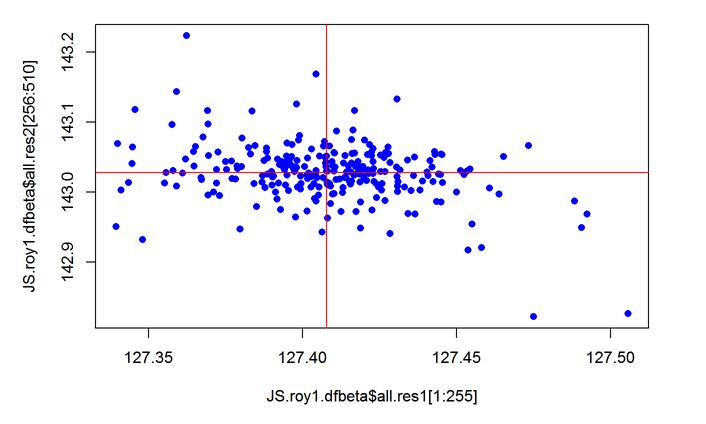
\includegraphics[width=0.7\linewidth]{images/dfbetas-JS-ROY}
		\caption{}
		\label{fig:dfbetas-JS-ROY}
	\end{figure}
	
%============================================================================= %
\section{Cooks's Distance - Implementation with \texttt{R}}
Cook's Distance is a measure indicating to what extent model parameters are influenced by (a set of) influential data on which the model is based. This function computes the Cook's distance based on the information returned by the \texttt{estex()} function.
	
%====================================================================================================%	

\section{residuals.lme {nlme}- Extract lme Residuals}

The residuals at level $i$ are obtained by subtracting the fitted levels at that level from the response vector (and dividing by the estimated within-group standard error, if \texttt{type="pearson"}). 

The fitted values at level i are obtained by adding together the population fitted values (based only on the fixed effects estimates) and the estimated contributions of the random effects to the fitted values at grouping levels less or equal to i.

%------------------------------------------------------------------------%

\begin{framed}
	\begin{verbatim}
	
	fm1 <- lme(distance ~ age + Sex, 
	data = Orthodont, random = ~ 1)
	head(residuals(fm1, level = 0:1))
	summary(residuals(fm1) /
	residuals(fm1, type = "p")) 
	
	# constant scaling factor 1.432
	
	\end{verbatim}
\end{framed}


	\chapter{Lesaffre's paper.}
\section{Lesaffre's paper.} %5.6

Lesaffre considers the case-weight perturbation approach.


%\citep{cook86}
Cook's 86 describes a local approach wherein each case is given a weight $w_{i}$ and the effect on the parameter estimation is measured by perturbing these weights. Choosing weights close to zero or one corresponds to the global case-deletion approach.

Lesaffre  describes the displacement in log-likelihood as a useful metric to evaluate local influence %\citep{cook86}.


%\citet{lesaffre}
Lesaffre describes a framework to detect outlying observations that matter in an LME model. Detection should be carried out by evaluating diagnostics $C_{i}$ , $C_{i}(\alpha)$ and $C_{i}(D,\sigma^2)$.


Lesaffre defines the total local influence of individual $i$ as
\begin{equation}
C_{i} = 2 | \triangle \prime _{i} L^{-1} \triangle_{i}|.
\end{equation}


The influence function of the MLEs evaluated at the $i$th point $IF_{i}$, given by
\begin{equation}
IF_{i} = -L^{-1}\triangle _{i}
\end{equation}
can indicate how $\hat{theta}$ changes as the weight of the $i$th
subject changes.

The manner by which influential observations distort the estimation process can be determined by inspecting the
interpretable components in the decomposition of the above measures of local influence.


Lesaffre comments that there is no clear way of interpreting the information contained in the angles, but that this doesn't mean the information should be ignored.




	\section{Lesaffre's paper.}
	Lesaffre considers the case-weight perturbation approach.
	
	
	\citep{cook86}
	Cook's 86 describes a local approach wherein each case is given a
	weight $w_{i}$ and the effect on the parameter estimation is
	measured by perturbing these weights. Choosing weights close to
	zero or one corresponds to the global case-deletion approach.
	
	Lesaffre  describes the displacement in log-likelihood as a useful
	metric to evaluate local influence %\citep{cook86}.
	
	%\citet{lesaffre}
	Lesaffre describes a framework to detect outlying observations
	that matter in an LME model. Detection should be carried out by
	evaluating diagnostics $C_{i}$ , $C_{i}(\alpha)$ and $C_{i}(D,
	\sigma^2)$.
	
	Lesaffre defines the total local influence of individual $i$ as
	\begin{equation}
		C_{i} = 2 | \triangle \prime _{i} L^{-1} \triangle_{i}|.
	\end{equation}
	
	The influence function of the MLEs evaluated at the $i$th point
	$IF_{i}$, given by
	\begin{equation}
		IF_{i} = -L^{-1}\triangle _{i}
	\end{equation}
	can indicate how $\hat{theta}$ changes as the weight of the $i$th
	subject changes.
	
	The manner by which influential observations
	distort the estimation process can be determined by inspecting the
	interpretable components in the decomposition of the above
	measures of local influence.
	
	
	Lesaffre comments that there is no clear way of interpreting the
	information contained in the angles, but that this doesn't mean
	the information should be ignored.
	%-----------------------------------------------------------------------------------------%
\section{influence.ME}

\textit{influence.ME} allows you to compute measures of influential data for mixed effects models generated by lme4.

\textit{influence.ME} provides a collection of tools for detecting influential cases in generalized mixed effects models. It analyses models that were estimated using lme4. The basic rationale behind identifying influential data is that when iteratively single units are omitted from the data, models based on these data should not produce substantially different estimates. 

To standardize the assessment of how influential a (single group of) observation(s) is, several measures of influence are common practice, such as DFBETAS and Cook's Distance. In addition, we provide a measure of percentage change of the fixed point estimates and a simple procedure to detect changing levels of significance.
\subsection{Influence() command}
\texttt{influence()} is the workhorse function of the influence.ME package. Based on a priorly estimated mixed effects regression model (estimated using lme4), the \texttt{influence()} function iteratively modifies the mixed effects model to neutralize the effect a grouped set of data has on the parameters, and which returns returns the fixed parameters of these iteratively modified models. These are used to compute measures of influential data.


\subsection{Classical Model}
The classical model is based on measurements $y_{mi}$
by method $m=1,2$ on item $i = 1,2 \ldots$

\[y_{mi} + \alpha_{m} + \mu_{i} + e_{mi}\]

\[e_{mi} \sim \mathcal{n} (0,\sigma^2_m)\]

Even though the separate variances can not be
identified, their sum can be estimated by the empirical variance of the differences.

Like wise the separate $\alpha$ can not be
estimated, only theiir difference can be estimated as
$\bar{D}$

\section{Lai Shiao}

\citet{LaiShiao} advocates the use of LME models to study method comparison problems. The authors analyse a data set typical of method comparison studies using SAS software, with particular use of the \emph{`Proc Mixed'} package. The stated goal of this study is to determine which factor from a specified group of factors is the key contributor to the difference in the two methods.

The study relates to oxygen saturation, the most investigated variable in clinical nursing studies \citep{LaiShiao}. The two method compared are functional saturation (SO2, percent functional oxy-hemoglobin) and fractional saturation (HbO2, percent fractional oxy-hemoglobin), which is considered to be the `gold standard' method of measurement.

\citet{LaiShiao} establishes an LME model for analysing the differences $D_{ijtl}$, where $D_{ijtl}$ is the differences of the measurements (i.e = $SO2_{ijtl}$ - $HbO2_{ijtl}$) for the ith donor at the $j$th level of foetal haemoglobin percent (Fhbperct) and the $t$th repeated measurement by the $l$th practitioner of the experiment.


(\citet{BXC2004} also advocates the use of LME models in comparing methods, but with a different emphasis.)
\citet{LaiShiao} use mixed models to determine the factors that
affect the difference of two methods of measurement using the
conventional formulation of linear mixed effects models.

If the parameter \textbf{b}, and the variance components are not
significantly different from zero, the conclusion that there is no
inter-method bias can be drawn. If the fixed effects component
contains only the intercept, and a simple correlation coefficient
is used, then the estimate of the intercept in the model is the
inter-method bias. Conversely the estimates for the fixed effects
factors can advise the respective influences each factor has on
the differences. It is possible to pre-specify different
correlation structures of the variance components \textbf{G} and
\textbf{R}.


Oxygen saturation is one of the most frequently measured variables
in clinical nursing studies. `Fractional saturation' ($HbO_{2}$)
is considered to be the gold standard method of measurement, with
`functional saturation' ($SO_{2}$) being an alternative method.
The method of examining the causes of differences between these
two methods is applied to a clinical study conducted by
\citet{Shiao}. This experiment was conducted by 8 lab
practitioners on blood samples, with varying levels of
haemoglobin, from two donors. The samples have been in storage for
varying periods ( described by the variable `Bloodage') and are
categorized according to haemoglobin percentages(i.e
$0\%$,$20\%$,$40\%$,$60\%$,$80\%$,$100\%$). There are 625
observations in all.

\citet{LaiShiao} fits two models on this data, with the lab
technicians and the replicate measurements as the random effects
in both models. The first model uses haemoglobin level as a fixed
effects component. For the second model, blood age is added as a
second fixed factor.

\subsubsection{Single fixed effect} The first model fitted by \citet{LaiShiao} takes the
blood level as the sole fixed effect to be analyzed. The following
coefficient estimates are estimated by `Proc Mixed';
\begin{eqnarray}
	\mbox{fixed effects :   } 2.5056 - 0.0263\mbox{Fhbperct}_{ijtl} \\
	(\mbox{p-values :   } = 0.0054, <0.0001, <0.0001)\nonumber\\\nonumber\\
	\mbox{random effects :   } u(\sigma^{2}=3.1826) + e_{ijtl}
	(\sigma^{2}_{e}=0.1525, \rho= 0.6978) \nonumber\\
	(\mbox{p-values :   } = 0.8113, <0.0001, <0.0001)\nonumber
\end{eqnarray}

With the intercept estimate being both non-zero and statistically
significant ($p=0.0054$), this models supports the presence
inter-method bias is $2.5\%$ in favour of $SO_{2}$. Also, the
negative value of the haemoglobin level coefficient indicate that
differences will decrease by $0.0263\%$ for every percentage
increase in the haemoglobin .

In the random effects estimates, the variance due to the
practitioners is $3.1826$, indicating that there is a significant
variation due to technicians ($p=0.0311$) affecting the
differences. The variance for the estimates is given as $0.1525$,
($p<0.0001$).

\subsubsection{Two fixed effects}
Blood age is added as a second fixed factor to the model,
whereupon new estimates are calculated;
\begin{eqnarray}
	\mbox{fixed effects :   } -0.2866 + 0.1072 \mbox{Bloodage}_{ijtl}
	- 0.0264\mbox{Fhbperct}_{ijtl}\nonumber\\
	( \mbox{p-values :   } = 0.8113, <0.0001, <0.0001)\nonumber\\\nonumber\\
	\mbox{random effects :   } u(\sigma^{2}=10.2346) + e_{ijtl}
	(\sigma^{2}_{e}=0.0920, \rho= 0.5577) \nonumber\\
	(\mbox{p-values :   } = 0.0446, <0.0001, <0.0001)
\end{eqnarray}


With this extra fixed effect added to the model, the intercept
term is no longer statistically significant. Therefore, with the
presence of the second fixed factor, the model is no longer
supporting the presence of inter-method bias. Furthermore, the
second coefficient indicates that the blood age of the observation
has a significant bearing on the size of the difference between
both methods ($p <0.0001$). Longer storage times for blood will
lead to higher levels of particular blood factors such as MetHb
and HbCO (due to the breakdown and oxidisation of the
haemoglobin). Increased levels of MetHb and HbCO are concluded to
be the cause of the differences. The coefficient for the
haemoglobin level doesn't differ greatly from the single fixed
factor model, and has a much smaller effect on the differences.
The random effects estimates also indicate significant variation
for the various technicians; $10.2346$ with $p=0.0446$.

\citet{LaiShiao} demonstrates how that linear mixed effects models
can be used to provide greater insight into the cause of the
differences. Naturally the addition of further factors to the
model provides for more insight into the behavior of the data.

\newpage
\chapter{Updating Techniques and Cross Validation}

\section{The Hat Matrix}
	The hat matrix, also known as the projection matrix, is well known in classical linear models. The diagonal elements $h_{ii}$ are known as `leverages'. The properties of $\boldsymbol{H}$  ,such as symmetry and idempotency, are well known.
	
	
	\begin{equation*}
		\boldsymbol{H} =  \boldsymbol{X(X^{\prime}X)^{-1}X^{\prime}}
	\end{equation*}
	
	
	\begin{equation*}
		\boldsymbol{H} = \left[%
		\begin{array}{cc}
			h_{ii} & \boldsymbol{h}^{\prime}_{i}\\
			\boldsymbol{h}_{i} & \boldsymbol{H}_{(i)}\\
		\end{array}%
		\right]
	\end{equation*}
	
	$\boldsymbol{H}_{(i)}$ is an $(n-1) \times (n-1)$ matrix. It's inversion for each $i$ is computationally expensive.
	
	\begin{equation*}
		\boldsymbol{C} = \boldsymbol{H}^{-1} =\left[%
		\begin{array}{cc}
			c_{ii} & \boldsymbol{h}^{\prime}_{c}\\
			\boldsymbol{c}_{i} & \boldsymbol{C}_{(i)}\\
		\end{array}%
		\right]
	\end{equation*}
	
\subsection{The Hat Matrix} %5.1

The projection matrix $H$ (also known as the hat matrix), is a
well known identity that maps the fitted values $\hat{Y}$ to the
observed values $Y$, i.e. $\hat{Y} = HY$.

\begin{equation}
H =\quad X(X^{T}X)^{-1}X^{T}
\end{equation}

$H$ describes the influence each observed value has on each fitted
value. The diagonal elements of the $H$ are the `leverages', which
describe the influence each observed value has on the fitted value
for that same observation. The residuals ($R$) are related to the
observed values by the following formula:
\begin{equation}
R = (I-H)Y
\end{equation}

The variances of $Y$ and $R$ can be expressed as:
\begin{eqnarray}
\mbox{var}(Y) = H\sigma^{2} \nonumber\\
\mbox{var}(R) = (I-H)\sigma^{2}
\end{eqnarray}

Updating techniques allow an economic approach to recalculating
the projection matrix, $H$, by removing the necessity to refit the
model each time it is updated. However this approach is known for
numerical instability in the case of down-dating.


\newpage
	\section{Efficient updating theorem}
	
	It is convenient to write partitioned matrices in which the $i$-th case is isolated. The partitioned matrix is written as $ i = 1$, but the results apply in general.
	
	%Tewomir pg 158
	If $\boldsymbol{C^{\prime}}_{i}  = [c_{ii}, \boldsymbol{c^{\prime}}_{i}]$, such that  $\boldsymbol{C}_{i}$ is the
	$i$-th column of $\boldsymbol{H}^{-1}$ then
	
	
	\begin{itemize}
		\item $m_{i} = \frac{1}{c_{ii}}$\\
		\item $\breve{x}_{i} = \frac{1}{c_{ii}}\boldsymbol{X^{\prime}C}_{i}$\\
		\item $\breve{\boldsymbol{z}_{ji}} = \frac{1}{c_{ii}}\boldsymbol{Z^{\prime}}_{j}\boldsymbol{C}_{i}$\\
		\item $\breve{y}_{i} = \frac{1}{c_{ii}}\boldsymbol{y^{\prime}C}_{i}$\\
	\end{itemize}
	
	Once $\boldsymbol{H}^{-1}$ is determined, an efficient updating formula can be applied.
	
	
	
	\begin{equation}
	\boldsymbol{H}^{-1} = \boldsymbol{I} - \boldsymbol{Z}(\boldsymbol{D}^{-1} + \boldsymbol{ZZ})^{-1}\boldsymbol{Z^{\prime}}
	\end{equation}
	
	
	%------------------------------------------------------------------------Chapter 6-----%
	\newpage
	%--------------------------------------------------------------%
	
	
	
	
	
	
\subsection{Updating Regression Estimates}
Let the observation $j$ be omitted from the data set. The estimates for the variance identities can be updating using minor adjustments to the full sample estimates. Where $(j)$ denotes that the $j$th has been omitted, these identities are

\begin{equation}
Sxx^{(j)}=\frac{\sum_{i=1}^{n}(x_{i}^{2})-(x_{j})^{2}-\frac{((\sum_{i=1}^{n}x_{i})-x_{j})^{2}}{n-1}}{n-2}
\end{equation}
\begin{equation}
Syy^{(j)}=\frac{\sum_{i=1}^{n}(y_{i}^{2})-(y_{j})^{2}-\frac{((\sum_{i=1}^{n}y_{i})-y_{j})^{2}}{n-1}}{n-2}
\end{equation}
\begin{equation}
Sxy^{(j)}=\frac{\sum_{i=1}^{n}(x_{i}y_{i})-(y_{j}x_{j})-\frac{((\sum_{i=1}^{n}x_{i})-x_{j})(\sum_{i=1}^{n}y_{i})-y_{k})}{n-1}}{n-2}
\end{equation}

The updated estimate for the slope is therefore
\begin{equation}
\hat{\beta}_{1}^{(j)}=\frac{Sxy^{(j)}}{Sxx^{(j)}}
\end{equation}

It is necessary to determine the mean for $x$ and $y$ of the remaining $n-1$ terms
\begin{equation}
\bar{x}^{(j)}=\frac{(\sum_{i=1}^{n}x_{i})-(x_{j})}{n-1},
\end{equation}

\begin{equation}
\bar{y}^{(j)}=\frac{(\sum_{i=1}^{n}y_{i})-(y_{j})}{n-1}.
\end{equation}

The updated intercept estimate is therefore

\begin{equation}
\hat{\beta}_{0}^{(j)}=\bar{y}^{(j)}-\hat{\beta}_{1}^{(j)}\bar{x}^{(j)}.
\end{equation}






\newpage



\subsection{Updating of Regression Estimates}
Updating techniques are used in regression analysis to add or delete rows from a model, allowing the analyst the effect of the observation associated with that row. In time series problems, there will be scientific interest in the changing relationship between variables. In cases where there a single row is to be added or deleted, the procedure used is equivalent to a geometric rotation of a plane.

Updating techniques are used in regression analysis to add or delete rows from a model, allowing the analyst the effect of the observation associated with that row.

Consider a $p \times p$ matrix $X$, from which a row $x_{i}^{T}$ is to be added or deleted. \citet{CookWeisberg} sets $A = X^{T}X$,
$a=-x_{i}^{T}$ and $b=x_{i}^{T}$, and writes the above equation as
	
	\begin{equation}
	(X^{T}X \pm x_{i}x_{i}^{T})^{-1} = \quad(X^{T}X )^{-1} \mp \quad
	\frac{(X^{T}X)^{-1}(x_{i}x_{i}^{T}(X^{T}X)^{-1}}{1-x_{i}^{T}(X^{T}X)^{-1}x_{i}}
	\end{equation}
	
This approach allows an economic approach to recalculating the
projection matrix, $V$, by removing the necessity to refit the
model each time it is updated.

This approach is known for numerical instability in the case of
downdating.
\subsection{Updating Standard deviation}
A simple, but useful, example of updating is the updating of the standard deviation when an observation is omitted, as practised in statistical process control analyzes. From first principles, the variance of a data set can be calculated using the following formula.
\begin{equation}
S^{2}=\frac{\sum_{i=1}^{n}(x_{i}^{2})-\frac{(\sum_{i=1}^{n}x_{i})^{2}}{n}}{n-1}
\end{equation}

While using bivariate data, the notation $Sxx$ and $Syy$ shall apply hither to the variance of $x$ and of $y$ respectively. The covariance term $Sxy$ is given by

\begin{equation}
Sxy=\frac{\sum_{i=1}^{n}(x_{i}y_{i})-\frac{(\sum_{i=1}^{n}x_{i})(\sum_{i=1}^{n}y_{i})}{n}}{n-1}.
\end{equation}

\subsection{Inference on intercept and slope}
	\begin{equation}
	\hat{\beta_{1}} \pm t_{(\alpha, n-2) }
	\sqrt{\frac{S^2}{(n-1)S^{2}_{x}}}
	\end{equation}
	
	\begin{equation}
	\frac{\hat{\beta_{0}}-\beta_{0}}{SE(\hat{\beta_{0}})}
	\end{equation}
	\begin{equation}
	\frac{\hat{\beta_{1}}-\beta_{1}}{SE(\hat{\beta_{0}})}
	\end{equation}


\subsection{Inference on correlation coefficient} This test of
the slope is coincidentally the equivalent of a test of the
correlation of the $n$ observations of $X$ and $Y$.
\begin{eqnarray}
H_{0}: \rho_{XY} = 0 \nonumber \\
H_{A}: \rho_{XY} \ne 0 \nonumber \\
\end{eqnarray}

%------------------------------------------------------------------------%

	\subsection{Sherman Morrison Woodbury Formula}
		
		The `Sherman Morrison Woodbury' Formula is a well known result in
		linear algebra;
		\begin{equation}
		(A+a^{T}B)^{-1} \quad = \quad A^{-1}-
		A^{-1}a^{T}(I-bA^{-1}a^{T})^{-1}bA^{-1}
		\end{equation}
		
		This result is highly useful for analyzing regression diagnostics,
		and for matrices inverses in general. Consider a $p \times p$
		matrix $X$, from which a row $x_{i}^{T}$ is to be added or
		deleted. \citet{CookWeisberg} sets $A = X^{T}X$, $a=-x_{i}^{T}$
		and $b=x_{i}^{T}$, and writes the above equation as
		
		\begin{equation}
		(X^{T}X \pm x_{i}x_{i}^{T})^{-1} = \quad(X^{T}X )^{-1} \mp \quad
		\frac{(X^{T}X)^{-1}(x_{i}x_{i}^{T}(X^{T}X)^{-1}}{1-x_{i}^{T}(X^{T}X)^{-1}x_{i}}
		\end{equation}
		

The projection matrix $H$ (also known as the hat matrix), is a
well known identity that maps the fitted values $\hat{Y}$ to the
observed values $Y$, i.e. $\hat{Y} = HY$.

\begin{equation}
H =\quad X(X^{T}X)^{-1}X^{T}
\end{equation}

$H$ describes the influence each observed value has on each fitted
	value. The diagonal elements of the $H$ are the `leverages', which
	describe the influence each observed value has on the fitted value
	for that same observation. The residuals ($R$) are related to the
	observed values by the following formula:
	\begin{equation}
		R = (I-H)Y
	\end{equation}
	
	The variances of $Y$ and $R$ can be expressed as:
	\begin{eqnarray}
		\mbox{var}(Y) = H\sigma^{2} \nonumber\\
		\mbox{var}(R) = (I-H)\sigma^{2}
	\end{eqnarray}
	
	Updating techniques allow an economic approach to recalculating
	the projection matrix, $H$, by removing the necessity to refit the
	model each time it is updated. However this approach is known for
	numerical instability in the case of down-dating.
	

\chapter{Appendices 1}


\section{Model Terms (Roy 2009)}
\begin{itemize}
	\item Let $y_{mir}$ be the response of method $m$ on the $i$th subject
	at the $r-$th replicate.
	\item Let $\boldsymbol{y}_{ir}$ be the $2 \times 1$ vector of measurements
	corresponding to the $i-$th subject at the $r-$th replicate.
	\item Let $\boldsymbol{y}_{i}$ be the $R_i \times 1$ vector of
	measurements corresponding to the $i-$th subject, where $R_i$ is number of replicate measurements taken on item $i$.
	\item Let $\alpha_mi$ be the fixed effect parameter for method for subject $i$.
	\item Formally Roy uses a separate fixed effect parameter to describe the true value $\mu_i$, but later combines it with the other fixed effects when implementing the model.
	\item Let $u_{1i}$ and $u_{2i}$ be the random effects corresponding to methods for item $i$.
	
	\item $\boldsymbol{\epsilon}_{i}$ is a $n_{i}$-dimensional vector
	comprised of residual components. For the blood pressure data $n_{i} = 85$.
	
	\item $\boldsymbol{\beta}$ is the solutions of the means of the two methods. In the LME output, the bias ad corresponding
	t-value and p-values are presented. This is relevant to Roy's first test.\end{itemize}


%---------------------------------------------------------------------------%

\section{Application to MCS} %4.1

Let $\hat{\beta}$ denote the least square estimate of $\beta$
based upon the full set of observations, and let
$\hat{\beta}^{(k)}$ denoted the estimate with the $k^{th}$ case
excluded.


\section{Grubbs' Data} %4.2

For the Grubbs data the $\hat{\beta}$ estimated are
$\hat{\beta}_{0}$ and $\hat{\beta}_{1}$ respectively. Leaving the
fourth case out, i.e. $k=4$ the corresponding estimates are
$\hat{\beta}_{0}^{-4}$ and $\hat{\beta}_{1}^{-4}$


\begin{equation}
Y^{-Q} = \hat{\beta}^{-Q}X^{-Q}
\end{equation}

When considering the regression of case-wise differences and averages, we write $D^{-Q} = \hat{\beta}^{-Q}A^{-Q}$


\newpage

\begin{table}[ht]
	\begin{center}
		\begin{tabular}{rrrrr}
			\hline
			& F & C & D & A \\
			\hline
			1 & 793.80 & 794.60 & -0.80 & 794.20 \\
			2 & 793.10 & 793.90 & -0.80 & 793.50 \\
			3 & 792.40 & 793.20 & -0.80 & 792.80 \\
			4 & 794.00 & 794.00 & 0.00 & 794.00 \\
			5 & 791.40 & 792.20 & -0.80 & 791.80 \\
			6 & 792.40 & 793.10 & -0.70 & 792.75 \\
			7 & 791.70 & 792.40 & -0.70 & 792.05 \\
			8 & 792.30 & 792.80 & -0.50 & 792.55 \\
			9 & 789.60 & 790.20 & -0.60 & 789.90 \\
			10 & 794.40 & 795.00 & -0.60 & 794.70 \\
			11 & 790.90 & 791.60 & -0.70 & 791.25 \\
			12 & 793.50 & 793.80 & -0.30 & 793.65 \\
			\hline
		\end{tabular}
	\end{center}
\end{table}

\begin{equation}
Y^{(k)} = \hat{\beta}^{(k)}X^{(k)}
\end{equation}

Consider two sets of measurements , in this case F and C , with the vectors of case-wise averages $A$ and case-wise differences $D$ respectively. A regression model of differences on averages can be fitted with the view to exploring some characteristics of the data.

When considering the regression of case-wise differences and averages, we write

\begin{equation}
D^{-Q} = \hat{\beta}^{-Q}A^{-Q}
\end{equation}
Let $\hat{\beta}$ denote the least square estimate of $\beta$ based upon the full set of observations, and let $\hat{\beta}^{(k)}$ denoted the estimate with the $k^{th}$ case excluded.

For the Grubbs data the $\hat{\beta}$ estimated are $\hat{\beta}_{0}$ and $\hat{\beta}_{1}$ respectively. Leaving the
fourth case out, i.e. $k=4$ the corresponding estimates are $\hat{\beta}_{0}^{-4}$ and $\hat{\beta}_{1}^{-4}$

\begin{equation}
Y^{(k)} = \hat{\beta}^{(k)}X^{(k)}
\end{equation}

Consider two sets of measurements , in this case F and C , with the vectors of case-wise averages $A$ and case-wise differences $D$ respectively. A regression model of differences on averages can be fitted with the view to exploring some characteristics of the data.

\begin{verbatim}
Call: lm(formula = D ~ A)

Coefficients: (Intercept)            A
-37.51896      0.04656

\end{verbatim}




When considering the regression of case-wise differences and averages, we write

\begin{equation}
D^{-Q} = \hat{\beta}^{-Q}A^{-Q}
\end{equation}

\section{Grubbs' data}
Let $\hat{\beta}$ denote the least square estimate of $\beta$ based upon the full set of observations, and let
	$\hat{\beta}^{(k)}$ denoted the estimate with the $k^{th}$ case excluded.
	
For the Grubbs data the $\hat{\beta}$ estimated are $\hat{\beta}_{0}$ and $\hat{\beta}_{1}$ respectively. Leaving the fourth case out, i.e. $k=4$ the corresponding estimates are $\hat{\beta}_{0}^{-4}$ and $\hat{\beta}_{1}^{-4}$
	
	\begin{equation}
	Y^{(k)} = \hat{\beta}^{(k)}X^{(k)}
	\end{equation}
	
	Consider two sets of measurements , in this case F and C , with the vectors of case-wise averages $A$ and case-wise differences $D$ respectively. A regression model of differences on averages can be fitted with the view to exploring some characteristics of the data.
	
	\begin{verbatim}
	Call: lm(formula = D ~ A)
	
	Coefficients: (Intercept)            A
	-37.51896      0.04656
	
	\end{verbatim}
	

	
	% latex table generated in R 2.9.2 by xtable 1.5-5 package
	% Wed Oct 21 14:04:18 2009
	\begin{table}[ht]
		\begin{center}
			\begin{tabular}{rrrrr}
				\hline
				& F & C & D & A \\
				\hline
				1 & 793.80 & 794.60 & -0.80 & 794.20 \\
				2 & 793.10 & 793.90 & -0.80 & 793.50 \\
				3 & 792.40 & 793.20 & -0.80 & 792.80 \\
				4 & 794.00 & 794.00 & 0.00 & 794.00 \\
				5 & 791.40 & 792.20 & -0.80 & 791.80 \\
				6 & 792.40 & 793.10 & -0.70 & 792.75 \\
				7 & 791.70 & 792.40 & -0.70 & 792.05 \\
				8 & 792.30 & 792.80 & -0.50 & 792.55 \\
				9 & 789.60 & 790.20 & -0.60 & 789.90 \\
				10 & 794.40 & 795.00 & -0.60 & 794.70 \\
				11 & 790.90 & 791.60 & -0.70 & 791.25 \\
				12 & 793.50 & 793.80 & -0.30 & 793.65 \\
				\hline
			\end{tabular}
		\end{center}
	\end{table}
	
	When considering the regression of case-wise differences and
	averages, we write
	
	\begin{equation}
	D^{-Q} = \hat{\beta}^{-Q}A^{-Q}
	\end{equation}
	
	\section{Grubb's example}
	For the Grubbs data the $\hat{\beta}$ estimated are $\hat{\beta}_{0}$ and $\hat{\beta}_{1}$ respectively. Leaving the
	fourth case out, i.e. $Q=4$ the corresponding estimates are $\hat{\beta}_{0}^{-4}$ and $\hat{\beta}_{1}^{-4}$
	
	\begin{equation}
	Y^{-Q} = \hat{\beta}^{-Q}X^{-Q}
	\end{equation}
	
	
	\section{Influence measures using R}
	R provides the following influence measures of each observation.
	
	%Influence measures: This suite of functions can be used to compute
	%some of the regression (leave-one-out deletion) diagnostics for
	%linear and generalized linear models discussed in Belsley, Kuh and
	% Welsch (1980), Cook and Weisberg (1982)
	
	\begin{table}[ht]
		\begin{center}
			\begin{tabular}{|c|c|c|c|c|c|c|}
				\hline
				& dfb.1\_ & dfb.A & dffit & cov.r & cook.d & hat \\
				\hline
				1 & 0.42 & -0.42 & -0.56 & 1.13 & 0.15 & 0.18 \\
				2 & 0.17 & -0.17 & -0.34 & 1.14 & 0.06 & 0.11 \\
				3 & 0.01 & -0.01 & -0.24 & 1.17 & 0.03 & 0.08 \\
				4 & -1.08 & 1.08 & 1.57 & 0.24 & 0.56 & 0.16 \\
				5 & -0.14 & 0.14 & -0.24 & 1.30 & 0.03 & 0.13 \\
				6 & -0.00 & 0.00 & -0.11 & 1.31 & 0.01 & 0.08 \\
				7 & -0.04 & 0.04 & -0.08 & 1.37 & 0.00 & 0.11 \\
				8 & 0.02 & -0.02 & 0.15 & 1.28 & 0.01 & 0.09 \\
				9 & 0.69 & -0.68 & 0.75 & 2.08 & 0.29 & 0.48 \\
				10 & 0.18 & -0.18 & -0.22 & 1.63 & 0.03 & 0.27 \\
				11 & -0.03 & 0.03 & -0.04 & 1.53 & 0.00 & 0.19 \\
				12 & -0.25 & 0.25 & 0.44 & 1.05 & 0.09 & 0.12 \\
				\hline
			\end{tabular}
		\end{center}
	\end{table}
	
	
	
	

	
	
\section{Sherman Morrison Woodbury Formula} % 5.2

The `Sherman Morrison Woodbury' Formula is a well known result in
linear algebra;
\begin{equation}
(A+a^{T}B)^{-1} \quad = \quad A^{-1}-
A^{-1}a^{T}(I-bA^{-1}a^{T})^{-1}bA^{-1}
\end{equation}

This result is highly useful for analyzing regression diagnostics,
and for matrices inverses in general. Consider a $p \times p$
matrix $X$, from which a row $x_{i}^{T}$ is to be added or
deleted. \citet{CookWeisberg} sets $A = X^{T}X$, $a=-x_{i}^{T}$
and $b=x_{i}^{T}$, and writes the above equation as

\begin{equation}
(X^{T}X \pm x_{i}x_{i}^{T})^{-1} = \quad(X^{T}X )^{-1} \mp \quad
\frac{(X^{T}X)^{-1}(x_{i}x_{i}^{T}(X^{T}X)^{-1}}{1-x_{i}^{T}(X^{T}X)^{-1}x_{i}}
\end{equation}

The projection matrix $H$ (also known as the hat matrix), is a
well known identity that maps the fitted values $\hat{Y}$ to the
observed values $Y$, i.e. $\hat{Y} = HY$.

\begin{equation}
H =\quad X(X^{T}X)^{-1}X^{T}
\end{equation}

$H$ describes the influence each observed value has on each fitted value. The diagonal elements of the $H$ are the `leverages', which describe the influence each observed value has on the fitted value for that same observation. The residuals ($R$) are related to the observed values by the following formula:
\begin{equation}
R = (I-H)Y
\end{equation}

The variances of $Y$ and $R$ can be expressed as:
\begin{eqnarray}
\mbox{var}(Y) = H\sigma^{2} \nonumber\\
\mbox{var}(R) = (I-H)\sigma^{2}
\end{eqnarray}

Updating techniques allow an economic approach to recalculating the projection matrix, $H$, by removing the necessity to refit the model each time it is updated. However this approach is known for
numerical instability in the case of down-dating.



\section{Hat Values for MCS regression}

With A as the averages and D as the casewise differences.
\begin{verbatim}
fit = lm(D~A)
\end{verbatim}

\begin{displaymath}
H = A \left(A^\top  A\right)^{-1} A^\top ,
\end{displaymath}

\chapter{Augmented GLMs} 


%---------------------------------------------------------------------------%
% - 3. Augmented GLMS
%---------------------------------------------------------------------------%


Generalized linear models are a generalization of classical linear  models.

\section{Augmented GLMs} %3.1

With the use of h-likihood, a random effected model of the form can be viewed as an `augmented GLM' with the response varaibkes $(y^t, \phi^t_m)^t$, (with $\mu = E(y)$,$ u = E(\phi)$, $var(y) = \theta V (\mu)$.
The augmented linear predictor is \[\eta_{ma}  = (\eta^t, \eta^t_m)^t) = T\omega. \].



%Augmented Generalized linear models.
% Youngjo et al page 154

The subscript $M$ is a label referring to the mean model.
\begin{equation}
\left(%
\begin{array}{c}
Y \\
\psi_{M} \\
\end{array}%
\right) = \left(
\begin{array}{cc}
X & Z \\
0 & I \\
\end{array}\right) \left(%
\begin{array}{c}
\beta \\
\nu \\
\end{array}%
\right)+ e^{*}
\end{equation}


%Augmented Generalized linear models.


The error term $e^{*}$ is normal with mean zero. The variance matrix of the error term is given by
\begin{equation}
\Sigma_{a} = \left(%
\begin{array}{cc}
\Sigma & 0 \\
0 & D \\
\end{array}%
\right).
\end{equation}

$y_{a} = T \delta + e^{*}$

Weighted least squares equation


% Youngjo et al page 154


\subsection{The Augmented Model Matrix}  %3.2
\begin{equation}
X = \left(%
\begin{array}{cc}
T & Z \\
0 & I \\
\end{array}%
\right)
\delta = \left(%
\begin{array}{c}
\beta  \\
\nu  \\
\end{array}%
\right)
\end{equation}





%-------------------------------------------------------------------------------------------------------------------------------------%
%-------------------------------------------------------------------------------------------------------------------------------------%
%-------------------------------------------------------------------------------------------------Chapter 4------------------------%
%-------------------------------------------------------------------------------------------------------------------------------------%
%-------------------------------------------------------------------------------------------------------------------------------------%



%------------------------------------------------%
\newpage

\section{Algorithms : ML v REML}
Maximum likelihood estimation is a method of obtaining estimates of unknown parameters by optimizing a likelihood function. The ML
parameter estimates are the values of the argument that maximise the likelihood function, i.e. the estimates that make the observed
values of the dependent variable most likely, given the distributional assumptions

The most common iterative algorithms used for the optimization
problem in the context of LMEs are the EM algoritm, fisher scoring
algorithm and NR algorithm, which [cite:West] commends as the
preferred method.

A mixed model is an extension of the general linear models that
can specify additional random effects terms.

Parameter of the mixed model can be estimated using either ML or
REML, while the AIC and the BIC can be used as measures of
"goodness of fit" for particular models, where smaller values are
considered preferable.

%--------------------------------------------------------------------%

(\textbf{\emph{Wikipedia}})The restricted (or residual, or reduced) maximum likelihood (REML) approach is a particular form of maximum likelihood estimation which does not base estimates on a maximum likelihood fit of all the information, but instead uses a likelihood function calculated from a transformed set of data, so that nuisance parameters have no effect.

In contrast to the earlier maximum likelihood estimation, REML can produce unbiased estimates of variance and covariance parameters.

%-----------------------------------------------------------------------------------------%

\noindent \textbf{ML procedures for LME}

The maximum likelihood procedure of Hartley and Rao yields
simultaneous estimates for both the fixed effects and the random
effect, by maximising the likelihood of $\boldsymbol{y}$ with
respect to each element of $\boldsymbol{\beta}$ and
$\boldsymbol{b}$.

%-----------------------------------------------------------------------------------------%
\newpage
\section{Estimation of random effects}

Estimation of random effects for LME models in the NLME package is accomplished through use
of both EM (Expectation-Maximization) algorithms and Newton-Raphson algorithms.
\begin{itemize}
	\item EM iterations bring estimates of the parameters into the region of the optimum very quickly, but
	convergence to the optimum is slow when near the optimum.
	\item Newton-Raphson iterations are computationally intensive and can be unstable when far from the
	optimum. However, close to the optimum they converge quickly.
	\item The LME function implements a hybrid approach, using 25 EM iterations to quickly get near the
	optimum, then switching to Newton-Raphson iterations to quickly converge to the optimum. \item If
	convergence problems occur, the ``control�argument in LME can be used to change the way the
	model arrives at the optimum.
\end{itemize}




%--Marginal and Conditional Residuals

\section{Covariance Parameters} %1.5
The unknown variance elements are referred to as the covariance parameters and collected in the vector $\theta$.
% - where is this coming from?
% - where is it used again?
% - Has this got anything to do with CovTrace etc?
%---------------------------------------------------------------------------%

\subsection{Methods and Measures}
The key to making deletion diagnostics useable is the development of efficient computational formulas, allowing one to obtain the \index{case deletion diagnostics} case deletion diagnostics by making use of basic building blocks, computed only once for the full model.

\citet{Zewotir} lists several established methods of analyzing influence in LME models. These methods include \begin{itemize}
	\item Cook's distance for LME models,
	\item \index{likelihood distance} likelihood distance,
	\item the variance (information) ration,
	\item the \index{Cook-Weisberg statistic} Cook-Weisberg statistic,
	\item the \index{Andrews-Prebigon statistic} Andrews-Prebigon statistic.
\end{itemize}
%--------------------------------------------------------------------------------------------%


\section{Haslett's Analysis} %2.5
For fixed effect linear models with correlated error structure Haslett (1999) showed that the effects on
the fixed effects estimate of deleting each observation in turn could be cheaply computed from the fixed effects model predicted residuals.


%---------------------------------------------------------------------------------------------------------%


\section{Computation and Notation } %2.3
with $\boldsymbol{V}$ unknown, a standard practice for estimating $\boldsymbol{X \beta}$ is the estime the variance components $\sigma^2_j$,
compute an estimate for $\boldsymbol{V}$ and then compute the projector matrix $A$, $\boldsymbol{X \hat{\beta}}  = \boldsymbol{AY}$.


\citet{Zewotir} remarks that $\boldsymbol{D}$ is a block diagonal with the $i-$th block being $u \boldsymbol{I}$




	\chapter{Generalized linear models}
	\section{Generalized Linear model}
	In statistics, the generalized linear model (GzLM) is a flexible
	generalization of ordinary least squares regression. The GzLM
	generalizes linear regression by allowing the linear model to be
	related to the response variable via a link function and by
	allowing the magnitude of the variance of each measurement to be a
	function of its predicted value.
	
	
	Mixed Effects Models offer a flexible framework by which to model
	the sources of variation and correlation that arise from grouped
	data. This grouping can arise when data collection is undertaken
	in a hierarchical manner, when a number of observations are taken
	on the same observational unit over time, or when observational
	units are in some other way related, violating assumptions of
	independence.
	
	\section{Generalized  Model(GzLM)}
	
	Nelder and Wedderburn (1972) integrated the previously disparate
	and separate approaches to models for non-normal cases in a
	framework called "generalized linear models."  The key elements of
	their approach is to describe any given model in terms of it's
	link function and it's variance function.
	
	\subsection{What is a GzLM}
	
	\begin{equation}
	\operatorname{E}(\mathbf{Y}) = \boldsymbol{\mu} =
	g^{-1}(\mathbf{X}\boldsymbol{\beta})
	\end{equation}
	
	where $E(Y)$ is the expected value of $Y$, $X\beta$ is the linear
	predictor, a linear combination of unknown parameters,$\beta$ and
	$g$ is the link function.
	
	
	$\operatorname{Var}(\mathbf{Y}) = \operatorname{V}(
	\boldsymbol{\mu} ) =
	\operatorname{V}(g^{-1}(\mathbf{X}\boldsymbol{\beta}))$
	\\
	
	
	\subsection{GzLM Structure}
	The GzLM consists of three elements. \\1. A probability
	distribution from the exponential family. \\2. A linear predictor
	$\eta= X\beta$ . \\3. A link function $g$ such that $E(Y)$ = $\mu$
	= $g^{-1}(eta)$.
	
	\subsection{Link Function}
	Definition 1 : The link function provides the relationship between
	the linear predictor and the mean of the distribution function.
	There are many commonly used link functions, and their choice can
	be somewhat arbitrary. It can be convenient to match the domain of
	the link function to the range of the distribution function's
	mean.
	
	\noindent Definition 2 : A link function is the function that
	links the linear model specified in the design matrix, where
	columns represent the beta parameters and rows the real
	parameters.
	
	\subsection{Canonical parameter}
	$\theta$, called the dispersion parameter,
	\subsection{Dispersion parameter}
	$\tau$, called the dispersion parameter, typically is known and is
	usually related to the variance of the distribution.
	
	\subsection{Iteratively weighted least square}
	IWLS is used to find the maximum likelihood estimates of a
	generalized linear model.
	
	\noindent Definition: An iterative algorithm for fitting a linear
	model in the case where the data may contain outliers that would
	distort the parameter estimates if other estimation procedures
	were used. The procedure uses weighted least squares, the
	influence of an outlier being reduced by giving that observation a
	small weight. The weights chosen in one iteration are related to
	the magnitudes of the residuals in the previous iteration — with a
	large residual earning a small weight.
	
	\subsection{Residual Components}
	In GzLMS the deviance is the sum of the deviance components
	
	\begin{equation}
	D = \sum d_{i}
	\end{equation}
	
	In GzLMS the deviance is the sum of the deviance components
	
	\newpage
	\section{Generalized linear mixed models}
	[pawitan section 17.8]
	
	The Generalized linear mixed model (GLMM) extend classical mixed models to non-normal outcome data.
	
	In statistics, a generalized linear mixed model (GLMM) is a particular type of mixed model. It is an extension to the
	generalized linear model in which the linear predictor contains random effects in addition to the usual fixed effects. These random effects are usually assumed to have a normal distribution.
	
	Fitting such models by maximum likelihood involves integrating over these random effects.
	
	
	
	%--------------------------------------------------------------------------------------%
	\newpage
	\chapter{LME Likelihood}
	\section{One Way ANOVA}
	\subsection{Page 448}
	Computing the variance of $\hat{\beta}$
	\begin{eqnarray}
	\mbox{var}(\hat{\beta}) = (X^{\prime}V^{-1}X)^-1
	\end{eqnarray}
	It is not necessary to compute $V^{-1}$ explicitly.
	
	\begin{eqnarray}
	V^{-1}X &= \Sigma^{1}{X-Z()Z^{\prime}\Sigma^{-1}X} \\
	&= \Sigma^{-1}(X-Zb_{x})
	\end{eqnarray}
	
	The estimate $b_{x}$ is the same term obtained from the random effects model; $X = Zb_{x} + e$, using $X$ as an outcome variable.
	This formula is convenient in applications where $b_{x}$ can be easily computed. Since $X$ is a matrix of $p$ columns, $b_{x}$ can simple be computed column by column. according to the columns of $X$.
	\subsection{Page 448- simple example}
	Consider a simple model of the form;
	\begin{equation*}
	y_{ij} = \mu + \beta_{i} + \epsilon_{ij}.
	\end{equation*}
	
	The iterative procedure is as follows Evaluate the individual group mean $\bar{y_{i}}$ and variance $\hat{Sigma^2}_{i}$. Then use the variance of the group means as an estimate of the $\sigma^2_{b}$. The average of the the variances of the groups is the initial estimate of the $\sigma^2_{e}$.
	\subsubsection{Iterative procedure}
	
	The iterative procedure comprises two steps, with $0$ as the first approximation of $b_{i}$.
	
	The first step is to compute $\lambda$, the ratio of variabilities,
	
	\begin{equation*}
	\lambda = \frac{\sigma^2_{b}}{\sigma^2_{e}}
	\end{equation*}
	
	\begin{eqnarray*}
		\mu = \frac{1}{N} \sum_{ij} (y_{ij} - b_{i}) \\
		b_{i} = \frac{n(\bar{y_{i}}-\mu)}{n+ \lambda} \\
	\end{eqnarray*}
	
	
	The second step is to updat $sigma^2_{e}$
	
	\begin{equation}
	\sigma^2_{e} = \frac{e^{\prime}e}{N-df}
	\end{equation}
	
	where $e$ is the vector of $e_{ij} = y_{ij}-\mu-b_{i}$ and $df =
	qn / n+\lambda$ and
	\begin{equation}
	\sigma^{2}_{b} = \frac{1}{q} \sum_{i=1}^{q} b_{1}^2 +
	(\frac{n}{\sigma^2_{e}}+\frac{1}{\sigma^2_{b}})^{-1}
	\end{equation}
	
	\subsubsection{Worked Example}
	
	Further to [pawitan 17.1] the initial estimates for variability
	are $\sigma^{2}_{b} = 1.7698$ and $\sigma^{2}_{e} = 0.3254$. At
	convergence the following results are obtained.
	\\
	n=16, q=5
	\begin{eqnarray*}
		\hat{\mu} = \bar{y} = 14.175 \\
		\hat{\sigma}^2 = 0.325\\
		\hat{\sigma}^2_{b} = 1.395\\
		\sigma  = 0.986 \\
	\end{eqnarray*}
	At convergene the following estimates are obtained,
	\begin{eqnarray*}
		\hat{\mu} = 14.1751 \\
		\hat{b}= (-0.6211, 0.2683,1.4389,-1.914,0.8279)\\
		\hat{\sigma}^2_{b} = 1.3955\\
		\hat{\sigma}^2_{e} = 0.3254\\
	\end{eqnarray*}
	
	
	\subsection{Extention to several random effects}
	[pawitan section 17.7]
	
	
	
	
	
	
	\section{Classical model for single measurements}
	The classical model is based on measurements $y_{mi}$
	by method $m=1,2$ on item $i = 1,2 \ldots$
	
	\[y_{mi} + \alpha_{m} + \mu_{i} + e_{mi}\]
	
	\[e_{mi} \sim \mathcal{n} (0,\sigma^2_m)\]
	
	Even though the separate variances can not be
	identified, their sum can be estimated by the empirical variance of the differences.
	
	Like wise the separate $\alpha$ can not be
	estimated, only theiir difference can be estimated as
	$\bar{D}$
	
	
	In the first instance, we require a simple model to describe a measurement by method $m$. We use the term $item$ to denote an individual, subject or sample, to be measured, being randomly sampled from a population. Let $y_{mi}$ be the measurement for item $i$ made by method $m$.
	
	\[ y_{mi} = \alpha_{m} + \mu_{i} + e_{mi}  \]
	
	\begin{itemize}
		\item $\alpha_m$ is the fixed effect associated with method $m$,
		\item $\mu_i$ is the true value for subject $i$ (fixed effect),
		\item $e_{mi}$ is a
		random effect term for errors with $e_{mi}  \sim \mathcal{N}(0,\sigma^2_m)$. \end{itemize}.
	
	This model implies that the difference between the paired measurements can be expressed as
	
	\[ d_{i} = y_{1i} - y_{2i} \sim \mathcal{N} (\alpha_{1} - \alpha_{2}, \sigma^2_{1} - \sigma^2_{2}). \]
	
	Importantly, this is independent of the item levels $\mu_i$. As the case-wise differences are of interest, the parameters of interest are the fixed effects for methods $\alpha_{m}$.
	
	\[ y_{mi} =  \alpha_{m}  + \mu_{i} + e_{mi}  \]
	
	
	
	
	
	Importantly these variance covariance structures are central to Roy methodology.
	
	
	\citet{Roy} proposes a series of hypothesis tests based on these matrices as part of her methodology. These tests shall be reverted to in due course.
	
	The standard deviation of the differences of variables $a$ and $b$ is computed as
	\[
	\mbox{var}(a - b) = \mbox{var} ( a )  + \mbox{var} ( b ) - 2\mbox{cov} ( a ,b )
	\]
	
	Hence the variance of the difference of two methods, that allows for the calculation of the limits of agreement, can be calculated as
	
	\[
	\mbox{var}(d) = \omega^2_1  + \omega^2_2 - 2 \times \omega_12
	\]
	
	
	
	
	
	\section{Sampling}
	\emph{
		One important feature of replicate observations is that they should be independent
		of each other. In essence, this is achieved by ensuring that the observer makes each
		measurement independent of knowledge of the previous value(s). This may be difficult
		to achieve in practice.} (Check who said this
	)
	
	
	
	
	
	
	\section{Limits of agreement in LME models}
	
	Limits of agreement are used extensively for assessing agreement, due to they're being intuitive and easy to use.
	Necessarily their prevalence in literature has meant that they are now the best known measurement for agreement, and that any newer methodology would benefit by making reference to them.
	
	\citet{BXC2008} uses LME models to determine the limits of agreement. Between-subject variation for method $m$ is given by $d^2_{m}$ and within-subject variation is given by $\lambda^2_{m}$.  \citet{BXC2008} remarks that for two methods $A$ and $B$, separate values of $d^2_{A}$ and $d^2_{B}$ cannot be estimated, only their average. Hence the assumption that $d_{x}= d_{y}= d$ is necessary. The between-subject variability $\boldsymbol{D}$ and within-subject variability $\boldsymbol{\Lambda}$ can be presented in matrix form,\begin{equation}
	\boldsymbol{D} = \left(%
	\begin{array}{cc}
	d^2_{A}& 0 \\
	0 & d^2_{B} \\
	\end{array}%
	\right)=\left(%
	\begin{array}{cc}
	d^2& 0 \\
	0 & d^2\\
	\end{array}%
	\right),
	\qquad \qquad
	\boldsymbol{\Lambda} = \left(%
	\begin{array}{cc}
	\lambda^2_{A}& 0 \\
	0 & \lambda^2_{B} \\
	\end{array}%
	\right).
	\end{equation}
	
	The variance for method $m$ is $d^2_{m}+\lambda^2_{m}$. Limits of agreement are determined using the standard deviation of the case-wise differences between the sets of measurements by two methods $A$ and $B$, given by
	\begin{equation}
	\mbox{var} (y_{A}-y_{B}) = 2d^2 + \lambda^2_{A}+ \lambda^2_{B}.
	\end{equation}
	Importantly the covariance terms in both variability matrices are zero, and no covariance component is present.
	
	\citet{BXC2008} presents a data set `fat', which is a comparison of measurements of subcutaneous fat
	by two observers at the Steno Diabetes Center, Copenhagen. Measurements are in millimeters
	(mm). Each person is measured three times by each observer. The observations are considered to be `true' replicates.
	
	A linear mixed effects model is formulated, and implementation through several software packages is demonstrated.
	All of the necessary terms are presented in the computer output. The limits of agreement are therefore,
	\begin{equation}
	0.0449  \pm 1.96 \times  \sqrt{2 \times 0.0596^2 + 0.0772^2 + 0.0724^2} = (-0.220,  0.309).
	\end{equation}
	
	\citet{roy} has demonstrated a methodology whereby $d^2_{A}$ and $d^2_{B}$ can be estimated separately. Also covariance terms are present in both $\boldsymbol{D}$ and $\boldsymbol{\Lambda}$. Using Roy's methodology, the variance of the differences is
	\begin{equation}
	\mbox{var} (y_{iA}-y_{iB})= d^2_{A} + \lambda^2_{B} + d^2_{A} + \lambda^2_{B} - 2(d_{AB} + \lambda_{AB})
	\end{equation}
	All of these terms are given or determinable in computer output.
	The limits of agreement can therefore be evaluated using
	\begin{equation}
	\bar{y_{A}}-\bar{y_{B}} \pm 1.96 \times \sqrt{ \sigma^2_{A} + \sigma^2_{B}  - 2(\sigma_{AB})}.
	\end{equation}
	
	For Carstensen's `fat' data, the limits of agreement computed using Roy's
	method are consistent with the estimates given by \citet{BXC2008}; $0.044884  \pm 1.96 \times  0.1373979 = (-0.224,  0.314).$
	
	\subsection{Linked replicates}
	
	\citet{BXC2008} proposes the addition of an random effects term to their model when the replicates are linked. This term is used to describe the `item by replicate' interaction, which is independent of the methods. This interaction is a source of variability independent of the methods. Therefore failure to account for it will result in variability being wrongly attributed to the methods.
	
	\citet{BXC2008} introduces a second data set; the oximetry study. This study done at the Royal Children?s Hospital in
	Melbourne to assess the agreement between co-oximetry and pulse oximetry in small babies.
	
	In most cases, measurements were taken by both method at three different times. In some cases there are either one or two pairs of measurements, hence the data is unbalanced. \citet{BXC2008} describes many of the children as being very sick, and with very low oxygen saturations levels. Therefore it must be assumed that a biological change can occur in interim periods, and measurements are not true replicates.
	
	\citet{BXC2008} demonstrate the necessity of accounting for linked replicated by comparing the limits of agreement from the `oximetry' data set using a model with the additional term, and one without. When the interaction is accounted for the limits of agreement are (-9.62,14.56). When the interaction is not accounted for, the limits of agreement are (-11.88,16.83). It is shown that the failure to include this additional term results in an over-estimation of the standard deviations of differences.
	
	Limits of agreement are determined using Roy's methodology, without adding any additional terms, are are found to be consistent with the 'interaction' model; $(-9.562, 14.504 )$. Roy's methodology assumes that replicates are linked. However, following Carstensen's example, an addition interaction term is added to the implementation of Roy's model to assess the effect, the limits of agreement estimates do not change. However there is a conspicuous difference in within-subject matrices of both models (denoted $1$ and $2$ respectively);
	\begin{verbatim}
	\begin{equation}
	\hat{\boldsymbol{\Lambda}}_{1}= \pmatrix{
	16.61 &	11.67\cr
	11.67 & 27.65 }\qquad
	\boldsymbol{\hat{\Lambda}}_{2}= \pmatrix{
	7.55 & 2.60 \cr
	2.60 & 18.59}
	\end{equation}
	\end{verbatim}
	
	The variance of the additional random effect in model $2$ is $3.01$.
	
	The Akaike information criterion (AIC) for both of models are $AIC_{1} = 2304.226$ and $AIC_{2} = 2306.226$. Having a difference of AIC values of $2$ is equivalent to both models being equally as good as the other. The AIC values for
	the Carstensen `unlinked' and `linked' models are $1994.66$ and $1955.48$ respectively.
	
	The $\boldsymbol{\hat{\Lambda}}$ matrices are informative as to the difference between Carstensen's unlinked and linked models. For the oximetry data, the covariance terms (given above as 11.67 and 2.6 respectively ) are of similar magnitudes to the variance terms. Conversely for the `fat' data the covariance term ($-0.00032$) is negligible. When the interaction term is added to the model, the covariance term remains negligible. (For the `fat' data, the difference in AIC values is also $2$).
	
	To conclude, Carstensen's models provided a rigorous way to determine limits of agreement, but don't provide for the computation of $\boldsymbol{\hat{D}}$ and $\boldsymbol{\hat{\Lambda}}$. Therefore the test's proposed by \citet{roy} can not be implemented. Conversely, accurate limits of agreement can be found using Roy's method.
	
	Addition of the interaction term erodes the capability of Roy's methodology to compare candidate models, and therefore shall not be adopted.
	
	(N.B. To complement the blood pressure `J vs S' analysis, the limits of agreement are $15.62 \pm 1.96 \times 20.33 = (-24.22, 55.46)$.)
	\newpage
	
	
	\section{Conclusion}
	\citet{BXC2008} and \citet{roy} highlight the need for method comparison methodologies suitable for use in the presence of replicate measurements. \citet{roy} presents a comprehensive methodology for assessing the agreement of two methods, for replicate measurements. This methodology has the added benefit of overcoming the problems of unbalanced data and unequal numbers of replicates. Implementation of the methodology, and interpretation of the results, is relatively easy for practitioners who have only basic statistical training. Furthermore, it can be shown that widely used existing methodologies, such as the limits of agreement, can be incorporated into Roy's methodology.
	%=========================================================================================================================================== %
	%=========================================================================================================================================== %
	
	\section*{9. Permutation Test, Power Tests and Missing Data }
	
	This section explores topics such as dependent variable simulation and power analysis, introduced by Galecki \& Burzykowski (2013), and implementable with their \textbf{\textit{nlmeU}} \texttt{R} package.
	Using the \textbf{\textit{predictmeans}} \texttt{R} package, it is possible to perform permutation t-tests for coefficients of (fixed) effects and permutation F-tests.
	
	The matter of missing data has not been commonly encountered in either Method Comparison Studies or Linear Mixed Effects Modelling. However Roy (2009) deals with the relevant assumptions regrading missing data. Galecki \& Burzykowski (2013) approaches the subject of missing data in LME Modelling. The \textbf{\textit{nlmeU}} package includes the \texttt{patMiss} function, which ``\textit{allows to compactly present pattern of missing data in a given vector/matrix/data
		frame or combination of thereof}".
	
	
	%================================================%
	
	\newpage
	\bibliographystyle{chicago}
	\bibliography{DB-txfrbib}
	
\end{document}


